\documentclass{article}
\usepackage{amsmath,amssymb,amstext,mathtools,array,url,bm,graphicx,color,epsfig}
\usepackage{fullpage,setspace}
\usepackage{authblk}
\usepackage{filecontents}
\usepackage{natbib}
\usepackage{lineno}
%\usepackage[colorlinks]{hyperref}
\usepackage{hyperref}
\usepackage{subcaption}
\usepackage{float}
\usepackage[flushleft]{threeparttable}

\newtheorem{theorem}{Theorem}
\newtheorem{acknowledgement}[theorem]{Acknowledgement}
\newtheorem{algorithm}[theorem]{Algorithm}
\newtheorem{axiom}[theorem]{Axiom}
\newtheorem{case}[theorem]{Case}
\newtheorem{claim}[theorem]{Claim}
\newtheorem{conclusion}[theorem]{Conclusion}
\newtheorem{condition}[theorem]{Condition}
\newtheorem{conjecture}[theorem]{Conjecture}
\newtheorem{corollary}[theorem]{Corollary}
\newtheorem{criterion}[theorem]{Criterion}
\newtheorem{definition}[theorem]{Definition}
\newtheorem{example}[theorem]{Example}
\newtheorem{exercise}[theorem]{Exercise}
\newtheorem{lemma}[theorem]{Lemma}
\newtheorem{notation}[theorem]{Notation}
\newtheorem{problem}[theorem]{Problem}
\newtheorem{proposition}[theorem]{Proposition}
\newtheorem{remark}[theorem]{Remark}
\newtheorem{solution}[theorem]{Solution}
\newtheorem{summary}[theorem]{Summary}
\newenvironment{proof}[1][Proof]{\noindent\textbf{#1.} }{\ \rule{0.5em}{0.5em}}

\begin{document}
\title{Probability modeling and uncertainty quantification of the Atenquique debris flow, 1955, M\'exico}
\author[1,2]{Andrea Bevilacqua}
\author[3,2]{Abani K. Patra}
\author[1]{Marcus I. Bursik}
\author[4]{E. Bruce Pitman}
\author[1]{David Hyman}
\author[5]{Ricardo Saucedo}
\author[6]{Jos\'e Luis Mac\'ias}

\affil[1]{\textit{Dept. of Earth Sciences, SUNY at Buffalo, NY 14260} }
\affil[2]{\textit{Comp. Data Science and Eng., SUNY at Buffalo, NY 14260} }
\affil[3]{\textit{Dept. of Mech. and  Aero. Eng., SUNY at Buffalo, NY 14260} }
\affil[4]{\textit{Dept. of Materials Design and Innovation, SUNY at Buffalo, NY, 14260}}
\affil[5]{\textit{Inst. de Geolog\'ia, Facultad de Ingenier\'ia, UASLP, SLP, 78240}}
\affil[6]{\textit{Dept. de Vulcanolog\'ia, Inst. de Geof\'isica, UNAM, DF, 04510}}

\date{\texttt{\{abevilac,abani,mib,pitman,davidhym\}@buffalo.edu},\\ \texttt{rgiron@uaslp.mx}, \texttt{macias@geofisica.unam.mx}}
\maketitle
\abstract
In this study we detail a new prediction-oriented procedure aimed at volcanic hazard assessment based on geophysical mass flow models with heterogeneous and poorly constrained output information. Our method relies on an itemized application of the empirical falsification principle over an arbitrarily wide envelope of possible input conditions. In particular, instead of fully calibrating input data on past observations, we create and explore input values under more general requirements of consistency, and then we separately use each piece of empirical data to remove those input values that are not compatible with it, hence defining partial solutions to the inverse problem. This has several advantages compared to a traditionally posed inverse problem: (i) the potentially non-empty intersection of the input spaces of partial solutions contains the solutions to the inverse problem; (ii) the partial solutions can provide hazard estimates under weaker constraints; (iii) if multiple models are applicable, specific performance scores against each piece of empirical information can be calculated. We apply our procedure to the case study of the Atenquique volcaniclastic debris flow, which occurred in the State of Jalisco (MX), 1955. We adopt and compare three depth averaged models currently implemented in the TITAN2D solver, available from vhub.org. The associated inverse problem is not well-posed if approached in a traditional way. However, we show that our procedure can extract valuable information for hazard assessment, allowing the exploration of the impact of model flows that are similar to those which occurred in the past, but differ in plausible ways.

\newpage
\section{Introduction}
The hazard assessment of geophysical mass flows usually relies on the reconstruction of past flows occurred in the area of interest. The available pieces of data $D_i$, $i\in I$ are commonly related to the properties of the deposit left by the flow, and to the historical documentation. In general, this information can be affected by relevant sources of uncertainty \citep{Hodgson1999, Pareschi2000}. Physical models provide us a relationship among inputs and outputs of the dynamical system of the mass flow \citep{Gilbert91}. In a probabilistic framework, for each model $M\in\mathcal M$ we define $\left(M, P_{M}\right)$, where $P_M$ is a probability measure over the parameter space of $M$.

While the support of $P_M$ can be restricted to a single value by solving an inverse problem for the optimal reconstruction of a particular flow, this is not always a well-posed problem \citep{Tarantola1982, Tarantola1987}. That is, no input data, or multiple input data, are able to produce outputs consistent with the observed information. Anyways, sometimes the strict replication of a past flow is not even desirable, especially if we are interested in the a general predictive capabilities of a model, where we are interested in the outcomes over a whole range. In this study we thus generalize a poorly constrained inverse problem, decomposing it into a hierarchy of simpler problems. Our purpose is to provide a new prediction-oriented formulation to use in hazard assessment problems.

\vskip.2cm Our approach is the following. 
\begin{enumerate}
\item For each model $M_j\in\mathcal M$, we initially set up a uniformly probabilized \emph{general input space} $(\Omega^j_0,\mathcal F_0^j, P^j_0)$ that we can define as arbitrary wide. At this stage we only require essential properties, namely the existence of the numerical output and the realism of the underlying physics. 
\item After a preliminary screening, we become able to characterize a \emph{specialized input space} $\Omega^j\subseteq\Omega^j_0$, under additional requirements which are related to the macroscopic properties of the outputs. For instance, a robust numerical simulation, a meaningful flow dynamics, and/or the capability to inundate a designated region.
\item Through more detailed testing, $\forall i\in I$, we can thus define the subspace $\Omega^j_i\subseteq\Omega^j$ of the inputs that are consistent with the piece of empirical data $D_i$.
\end{enumerate}
All these subspaces, if not negligible, are trivially probabilized by the push-forward measure of their inclusion in $\Omega^j_0$, up to the multiplicative constant $P^j_0(\Omega^j_i)$, $\forall i,j$.

\vskip.2cm The philosophy of our method is based on a itemized application of the empirical falsification principle of Karl R. Popper, over an arbitrary wide envelope of possible input conditions. The construction of the subspaces $(\Omega^j_i)_{i\ge1}$ has several advantages compared to a traditionally posed inverse problem:
\begin{itemize}
  \item the intersection space $\Theta^j:=\bigcap_i \Omega^j_i$ describes the set of the inputs that solve the inverse problem;
  \item the partial solutions $(\Omega^j_i)_{i\ge1}$ can provide information concerning flows that are partially solving the inverse problem, and they may exist even if $\Theta^j=\emptyset$;
  \item each probability $P(\Omega^j_i)$ represents a performance score of the adopted model against the piece of empirical data $D_i$, and can hence be used for model selection purposes.
\end{itemize}

\vskip.2cm We apply our procedure to the case study of the Atenquique volcaniclastic debris flow, occurred in the State of Jalisco (MX), 1955. We adopt and compare the three depth averaged models \emph{Mohr-Coulomb} (MC) \citep{SavageHutter1989}, \emph{Pouliquen-Forterre} (PF) \citep{Pouliquen1999, ForterrePouliquen2002, PouliquenForterre2002} and \emph{Voellmy-Salm} (VS) \citep{Voellmy1955, Salm1990}, based on the Saint-Venant equations. Input spaces are explored by Monte Carlo simulation based on Latin Hypercube sampling \citep{McKay1979,Owen1992b,Stein1987,Ranjan2014,Mingyao2016}. The three models are incorporated in our large scale mass flow simulation framework  TITAN2D \citep{Patra2005,Patra2006, Yu2009, Aghakhani2016}. So far, TITAN2D has been successfully applied to the simulation of different geophysical mass flows with specific characteristics \citep{Sheridan2005, Rupp2006, Norini2008, Charbonnier2009, Procter2010, Sheridan2010, Sulpizio2010, Capra2011}. Several studies involving TITAN2D were also directed towards a statistical study of geophysical flows, focusing on uncertainty quantification \citep{Dalbey2008, Dalbey2009, Stefanescu2012b, Stefanescu2012a}, or on the more efficient production of hazard maps \citep{Bayarri2009, Spiller2014, Bayarri2015, Ogburn2016}.

This is the summary of the study: in section \ref{s1} we present the Atenquique case study; in section \ref{s2} we introduce the physical models implemented, we define and parameterize the input spaces, and we design the Monte Carlo simulation; in section \ref{s3} we statistically describe the characteristics of the outputs and contributing variables, mapping them globally and detailing them locally; in section \ref{s4} we calculate the likelihood of multiple pieces of information regarding the 1955 debris flow, we use them to condition the input space, and then we compare the performances of the models over that space. We show that only VS model can provide a not empty $\Theta^j$, containing multiple solutions to the inverse problem.

\section{Nevado de Colima volcano and Barranca de Atenquique}\label{s1}
The Colima Volcanic Complex is located in the western portion of the Trans-Mexican Volcanic Belt (small box in Fig. 1). It consists of a N�S volcanic chain formed by C\'antaro, Nevado de Colima, and Colima volcanoes within the Colima Graben \citep{Luhr1990}. It began forming 1.7 Ma ago with the growth of C\'antaro Volcano, and continued with the formation of Nevado de Colima volcano 0.53 Ma ago \citep{Robin1987}. Activity was intermittent during the Pleistocene and Holocene and continues today at Colima volcano south of the Nevado de Colima \citep{Saucedo2010, Zobin2015, Macorps2018}.

Nevado de Colima (4320 m.a.s.l.) occupies the central part of the volcanic complex, being the most voluminous of the volcanoes (300�-400 km$^3$). It is characterized by three horseshoe-shaped craters. The youngest crater is 4 km wide and opens to the east with 100 m thick vertical walls. This structure contains the summit Picacho dome (4300 m). The eastern flank of Nevado de Colima volcano exposes a thick sequence of debris flows, fluvial, pyroclastic flow and debris avalanche deposits known as the Atenquique Formation \citep{Mooser1961, Saucedo2008}, covered by younger deposits of Nevado de Colima Volcano. The caldera morphology directs a large part of the drainage from the volcano into the Atenquique ravine, located on the ENE flank of the volcano and $\sim$25 km long. Figure 1 shows the ravine and its surrounding topography. Plot (\ref{Fig1}b) includes elevation isolines from the SRTM DEM of 30 m cell-size, UTM Zone 13N \citep{NASA2014}. The drainage begins at an elevation of 4000 m on the eastern flank of Nevado de Colima, is occupied by the perennial Atenquique river, and ends at its junction with the perennial Tuxpan River at 1040 m. Between, 4000 and 2000 m in altitude, the ravine has an average slope of 34$^\circ$. At an elevation of 1800 m, the Atenquique ravine is cut off by a 250 m cliff in the vicinity of the junction with the Dos Volcanes dry ravine (Fig 1). Beyond this cliff, the slope of the ravine suddenly decreases from 34$^\circ$ to 18$^\circ$, keeping this gradient to an elevation of 1600 m at 11.5 km from the NCV summit. Between this site and the catchments of the Los Pl\'atanos and Arroyo Seco dry ravines, located at $\sim$21.5 km at an elevation of 1120 m, the ravine gradient varies from 10$^\circ$ to 6$^\circ$. The town of Atenquique is located at an altitude of 1050 m, and 18.5 km (25 km along the ravine path) from the head of the ravine, where the ravine channel has a gradient of 5$^\circ$, that is maintained down to the confluence with the Tuxpan River (Fig. \ref{Fig1}). Atenquique ravine has an average width of 30 m, although in the vicinity of the Atenquique village it is up to 200 m wide.

\subsection{The Atenquique volcaniclastic debris flow, 1955}
On October 16, at 10:45 am, the inhabitants of Atenquique described the sudden arrival of a 8�9 m high wave carrying mud, boulders and tree trunks that devastated the buildings in the town and four bridges, including the railroad bridge. More than 23 people died, and the flood leveled everything but the tower of the church and the upper part of the market place that luckily served as shelter for survivors \citep{PonceSegura1983, Saucedo2008}. During the peak flow, eyewitnesses observed that complete walls of buildings were displaced several meters by the flood prior to their collapse. The deposits are exposed along the Atenquique, Arroyo Seco, Los Pl\'atanos and Dos Volcanes ravines, and their distribution, stratigraphy, granulometry, and volume have been recently described in \cite{Saucedo2008}. Sixty stratigraphic sections were studied along the Atenquique ravine and its main tributaries, and are reported as red dots and yellow stars in Figure 1. Deposits cover a minimal area of 1.2 km$^2$, and with an average thickness of 4 m, a minimum volume of 3.2$\times10^6$ m$^3$ was estimated for the flow.

The main flood probably formed in the Atenquique ravine, but enhanced by the confluence of flows from its tributaries: Dos Volcanes at 11.2 km, Arroyo Seco and Los Pl\'atanos, at 22.5 km. During the first 10 km (as recorded by the proximal exposures) the flow moved down steep slopes, eroding and incorporating coarse alluvium and sand. Downstream, in the medial exposures, the flow encountered gentler slopes, reducing its velocity and promoting deposition of part of the sediment load. Just before the village, below the junction with the Arroyo Seco and Los Pl\'atanos ravines, eyewitnesses reported peak flood levels, possibly enhanced by the engulfing of a small water reservoir. At the junction, the flow captured the fine-material load of flow from the Arroyo Seco and Pl\'atanos ravines, causing significant dilution and a sudden increase in the flow turbulence. Downstream the town, the flow lost its capacity to transport large boulders, probably due to widening of the reach and the consequent fall in velocity, which was further reduced by the hydraulic roughness effects of flow impacting buildings. The diluted flow probably had a velocity in the range of 4 to 6 m/s, obtained by comparison with analog flows \citep{Pierson1985, Saucedo2008}. The flood finally continued downstream to join with the perennial Tuxpan River, where emplaced up to 6 m of deposits.

\begin{figure}[H]
\centering
\includegraphics[width=1\textwidth]{Fig1.jpg}
\caption{Barranca de Atenquique (M{\'e}xico) overview. (a) Stratigraphic sections of \citep{Saucedo2008} are marked with red dots, including 5 preferred locations (stars) and major ravines. Shaded sites are detailed in Supporting Information. Initial source piles are marked by blue dots. Coordinates and projection are UTM zone 13N. (b) Digital elevation map including isolines \citep{NASA2014}. Volume partition percentages among sources are reported. Regional geology map is included in a small box.}
\label{Fig1}
\end{figure}

\subsection{Multiple sources and their locations}
The 1955 debris flow, according to eyewitness accounts and deposit analyses, emanated from multiple sources throughout the watershed. The existence of multiple source areas presents a unique challenge when attempting to model this flow. Eyewitnesses confirm that after the event, many small landslides scars were present along the main ravine and its tributaries. It is hypothesized that numerous small-volume landslides, triggered by rain infiltration, supplied the bulk of the material \citep{Saucedo2003}. To account for this, basing on the work in \cite{Rupp2004} we establish to initiate the flow from five major source locations, reported in Fig. \ref{Fig1}. We remark that our numerical simulation allows for multiple starting points in the same run. Each source consists in a paraboloid pile of material with unitary aspect ratio.

Two source locations (\#1 and \#2) are placed in the main ravine, one (\#3) in the a lateral valley associated with the regional Tamazula fault, one source (\#4) in Arroyo Seco and one (\#5) in Arroyo Pl\'atanos. These locations are selected based upon local topography. The first three are located on steep upland slopes, while the other two are located along the main drainage due to the lack of steep terrain nearby \citep{Rupp2004}.

The partition of volume $V=\sum^5_{k=1} V_k$ among the five sources is scaled based upon the size of the drainage basin they are located within. In particular, $\forall k$ we define $w_k=V_k/V$ as:
$$w_1=w_3=w_4=19.24\%, \quad w_2=37.58\%, \quad w_5=4.70\%.$$
This is equivalent to choose pile radii proportional to $80\ m$, $100\ m$ and $50\ m$ respectively.

We remark that source number, locations, and volume partition will be preserved in the following analysis. However, we tested that small variations are affecting the character of the simulated flow only proximally. Large variations would require additional field work to be justified, and are beyond the purpose of this study. More details about volume $V$ are provided in Section \ref{sub2.1}.

\section{Geophysical mass flow modeling in a prediction-oriented framework}\label{s2}
Our numerical modeling of the Atenquique flow proceeds by first assuming that the laws of mass and momentum conservation hold for properly defined system boundaries. The flow had very small depth compared to its length, and hence we assumed to integrate through the depth to obtain simpler and more computationally tractable equations \citep{SavageHutter1989}. The depth-averaged Saint-Venant equations that result are:
\begin{eqnarray}
\label{eq:D_A}
\frac{\partial h}{\partial t} +
\frac{\partial}{\partial x}(h \bar{u}) +
\frac{\partial}{\partial y}(h\bar{v}) &=& 0 \nonumber \\
\frac{\partial}{\partial t} (h\bar{u}) +
\frac{\partial}{\partial x}\left(h\bar{u}^2 + \frac{1}{2}k g_{z}h^2\right) + \frac{\partial}{\partial y}(h\bar{u}\bar{v}) &=& S_{x}\\
\frac{\partial}{\partial t} (h\bar{v}) +
\frac{\partial}{\partial x}(h\bar{u}\bar{v}) +
\frac{\partial}{\partial y}\left(h\bar{v}^2 + \frac{1}{2}k g_{z}h^2\right) &=& S_{y} \nonumber
\end{eqnarray}
Here the Cartesian coordinate system is aligned such that $z$ is normal to the surface; $h$ is the flow height in the $z$ direction; $h\bar{u}$ and $h\bar{v}$ are respectively the components of momentum in the $x$ and $y$ directions; and $k$ is the coefficient which relates the lateral stress components, $\bar{\sigma}_{xx}$ and $\bar{\sigma}_{yy}$, to the normal stress component, $\bar{\sigma}_{zz}$. Note that $\frac{1}{2} k g_z h^2$ is the contribution of hydrostatic pressure to the momentum fluxes. $S_x$ and $S_y$ are the sum local stresses: their definition depends on the constitutive model of the flowing material we choose. They include the gravitational driving forces, the basal friction force resisting to the motion of the material, and additional forces specific of rheology assumptions.

I this study we adopted the \emph{Mohr-Coulomb} (MC), \emph{Pouliquen-Forterre} (PF) and \emph{Voellmy-Salm} (VS) models, detailed in Appendix  \ref{A-1}. These three models for large scale mass flows are incorporated in our large scale mass flow simulation framework  TITAN2D \citep{Patra2005,Patra2006, Yu2009, Aghakhani2016}. The $\mathrm{4^{\mathrm{th}}}$ release of TITAN2D \footnote{available from vhub.org} offers multiple rheology options in the same code base \citep{Patra2018}. The availability of three distinct models for similar phenomena in the same tool provides us the ability to directly compare  outputs and internal variables in all the three models and control for usually difficult to quantify effects like numerical solution procedures, input ranges and computer hardware.

\subsection{Preliminary definition of the input space}\label{sub2.1}
The definition of the input space hierarchy $\mathbb R_+^{d_j}\supseteq\Omega_0^j\supseteq\Omega^j\supseteq\Omega^j_i$, $\forall i,j$, is a fundamental part of our approach. The dimensionality $d_j$ is a characteristic of the model. The input spaces of MC and VS have three dimensions so parameterized:
$$\Omega_0^{\mathrm{MC}} = \left\{(\phi_{bed}, \phi_{int}, V)\in \mathbb R_+^3\right\},$$
$$\Omega_0^{\mathrm{VS}} = \left\{(\arctan(\mu),\log_{10}(\xi),V)\in \mathbb R_+^3\right\}.$$
Instead, the input space of model PF originally has six dimensions - $(\phi_1, \phi_2, \phi_3, \beta, L, V)$. Following \cite{PouliquenForterre2002}, we constrain $\phi_3=\phi_1+1^\mathrm{\circ}$. Moreover, preliminary testing in our case study showed an equivalent impact from the variation of $\beta$ an $L$. So, we were able to further reduce $d_{\mathrm{PF}}=4$ by assuming the empirical relationship:
\begin{equation}
\beta=f(\phi_2):=\frac{\phi_2 - 7^\circ}{20} + 0.1,
\end{equation}
which is not restrictive, and consistent with the $\beta$ values presented in literature \citep{PouliquenForterre2002, ForterrePouliquen2003}. We thus effectively parameterize:
$$\Omega_0^{\mathrm{PF}} = \left\{(\phi_1, \phi_2, L, V)\in \mathbb R_+^4\right\}.$$

\subsubsection{General input space}
The input space boundaries of $\Omega_0^j$ are naturally constrained by some general assumptions, listed below.
\begin{itemize}
\item \textbf{Total Volume:} $V\in[3.5,\ 5] \times 10^6\ m^3$, i.e. $4.25 \pm 0.75$ $\times 10^6\ m^3$.
\item \textbf{Input space constraints:}
\par\noindent \textbf{MC} - $\phi_{bed} \ge 5^\circ$, $\quad \phi_{int} \in [\phi_{bed},\ 45^\circ]$.

\vskip.1cm\noindent \textbf{PF} - $\phi_1 \ge 1^\circ$, $\quad \phi_2 \in [\phi_1+6^\circ,\ \phi_1+18^\circ]$, $\quad L \in [0.1\ m,\ 0.5\ m]$.

\vskip.1cm\noindent \textbf{VS} - $\arctan(\mu)\ge 1^\circ$, $\quad \log_{10}(\xi)\le 4$.
\end{itemize}
In particular, a minimum volume of $3.2 \times 10^6\ m^3$ for the deposit left by the flow was obtained by \cite{Saucedo2008}. We assumed to increase it of about 10\% to 50\% to represent the volume of the simulated flow. We exclude basal friction angles below $5^\circ$ in MC, and $1^\circ$ in PF and VS because of evident numerical instability and unphysical behavior. In MC we constrain $\phi_{bed}<\phi_{int}$, and we exclude internal friction over $45^\circ$ because not realistic. In VS we do not allow $\xi$ over $10^4$ because producing unphysical results. In PF we constrain  $\phi_1+6^\circ<\phi_2<\phi_1 + 18^\circ$, extending the intervals of values presented in literature \citep{PouliquenForterre2002, ForterrePouliquen2003}. Then, parameter $L$ is related to the particle size \cite{ForterrePouliquen2003}, and hence we restrict it to be consistent with the observed average clasts sampled in the field \citep{Saucedo2008}.

\subsubsection{Specialized input space}
The construction of $\Omega_0^j$ relies on extensive testing of the models over the general input space defined above. We based our analysis on two qualitative properties that any realistic and hazardous flow must have: (i) the flow reaches the town of Atenquique in a reasonable time, (ii) the flow does not run-up and over-spill the ravine walls. We quantitatively re-formulated them as
\begin{itemize}
\item[(i)] the flow has reached a minimum elevation $h<1200$ m a.s.l. at $t=1200$ s,
\item[(ii)] the over-spill at the confluence of flow from sources \#1 and \#2, or \#1 + \#2 and \#3, is $<0.1$ m height.
\end{itemize}
We selected such elevation because it is about 1 km before the village \citep{Saucedo2008}, and we chosen $t=1200$ s because we observed that slower flows are not able to realistically inundate the village. We focused on those confluences because they are where the major over-spill issues take place in our tests.

Table 1 reports data of minimum elevation at $1200$ s, and over-spill issues. These values concern a flow volume $V=4.18\times 10^6$ $m^3$, roughly equivalent to the mean value of our range. Following the empirical falsification principle, we snip the input range by the deletion of those region which do not satisfy our requirements. The obtained subspaces have not rectangular shape, but look like parallelograms - this is because the effects of the input variables on the output are not independent.

\begin{figure}[H]
\centering
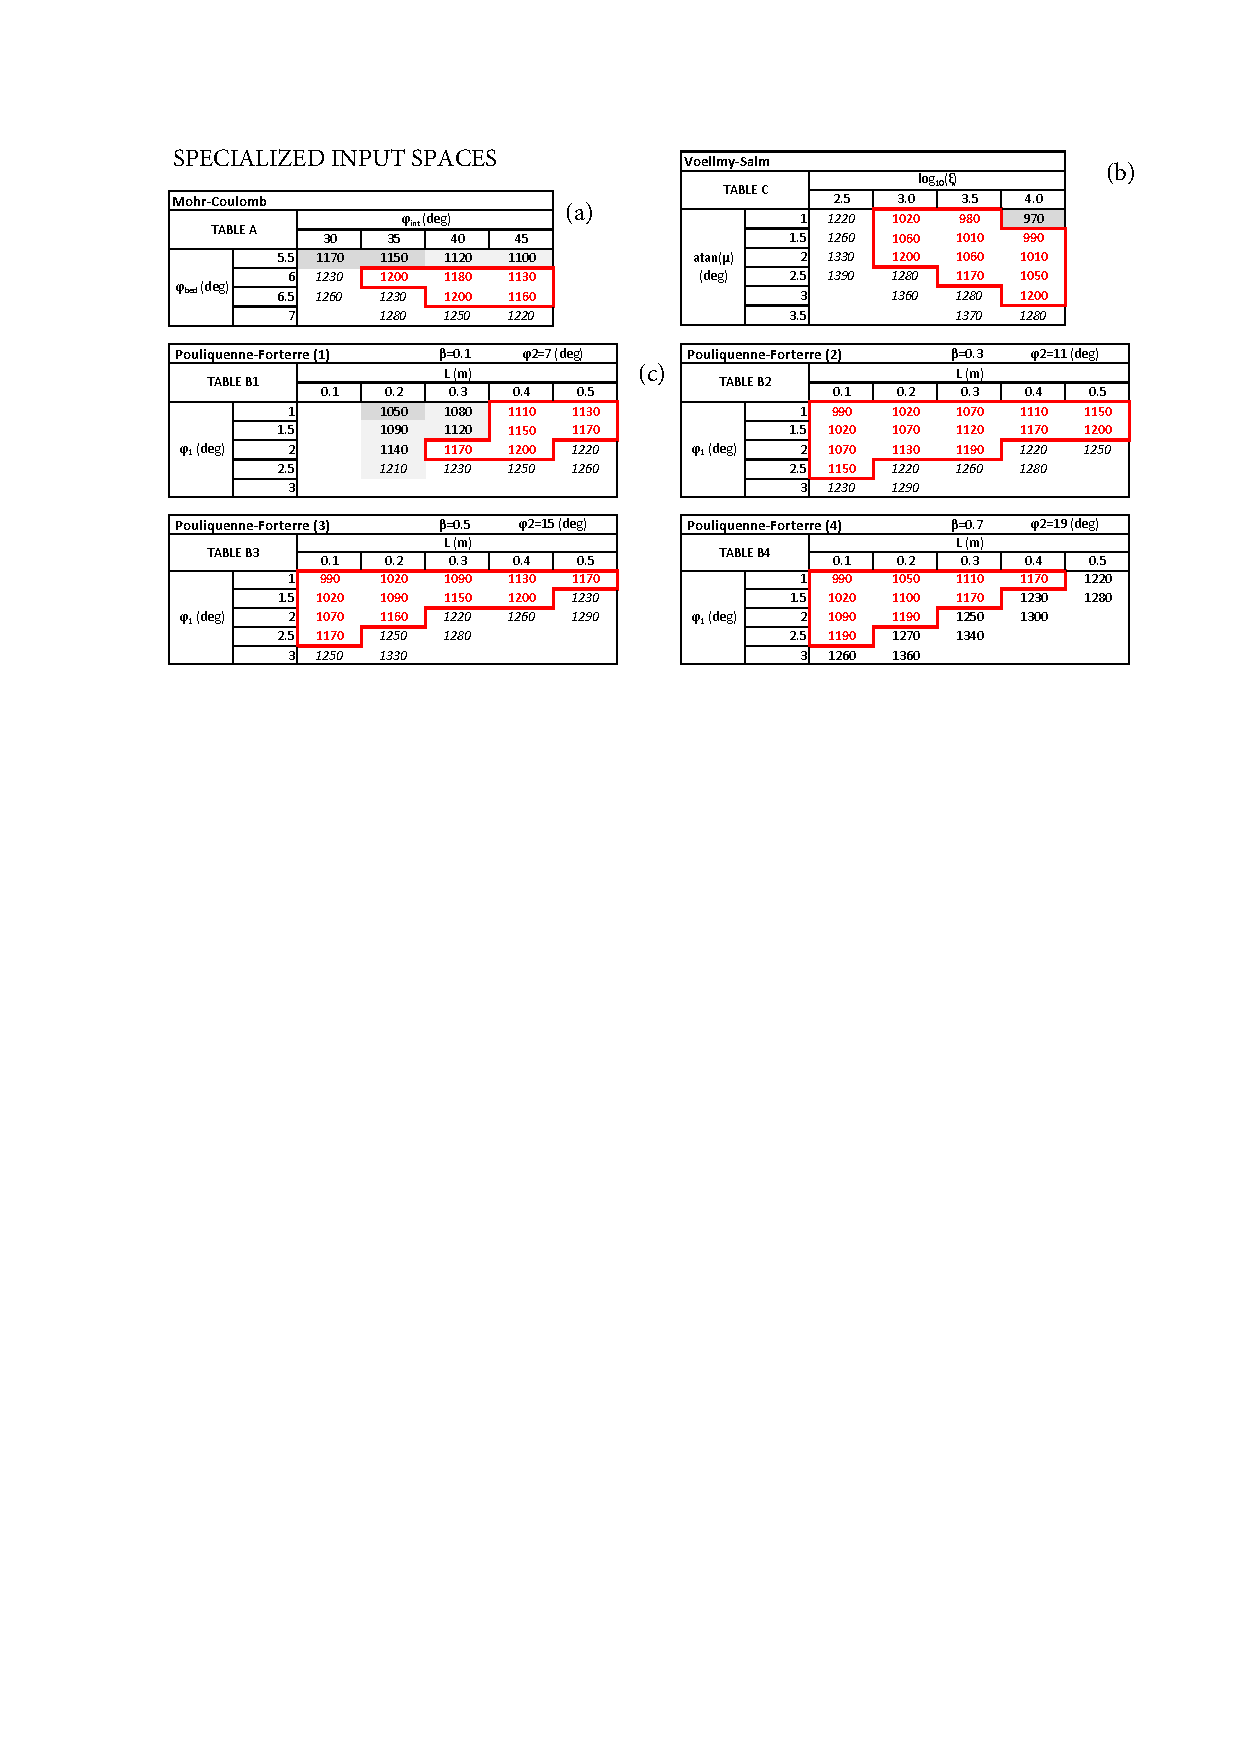
\includegraphics[width=1\textwidth]{Table1.pdf}
\caption*{Table 1: Input space explorative testing of (a) MC, (b) VS, (c) PF models, $V=4.18\times 10^6$ $m^3$. The 3D input space of PF is described by four 2D subspaces. Values reported are the minimum elevation $h$ reached at $t=1200$ s. A gray background marks those inputs that generate unphysical flow run-up and over-spill the ravine walls, light gray if $>0.1$ m, dark gray if $>1$ m. Red lines mark $\Omega^j$ subdomain of flows with $h\le1200$ m and without over-spill issues.}
\end{figure}

\begin{itemize}
\item In MC we observe over-spill issues for any $\phi_{bed} < 6^\circ$, and a too short runout for any $\phi_{bed} > 6.5^\circ$. We also note an increase of the runout if increasing the values of $\phi_{int}$. In particular, $\phi_{int} \ge 35^\circ$ is required to inundate the village.
\item In VS the over-spill is observed in the region $\{\arctan(\mu)<1.5^\circ\} \times \{\log_{10}(\xi)>3.5\}$. In contrast, the region $\{\arctan(\mu)>3^\circ\} \times \{\log_{10}(\xi)<3\}$ produces a too short runout.
\item Model PF must be treated in more detail because of its higher dimensionality. We cut it on four different hyperplanes corresponding to different values of $\phi_2$ and $\beta=f(\phi_2)$. Over-spill was observed only in the slice with $\phi_2=7^\circ$, and only for $L<0.4$ m. In general, $\phi_1<3^\circ$ is required to have a long-enough run-out.
\end{itemize}

\begin{figure}[H]
\centering
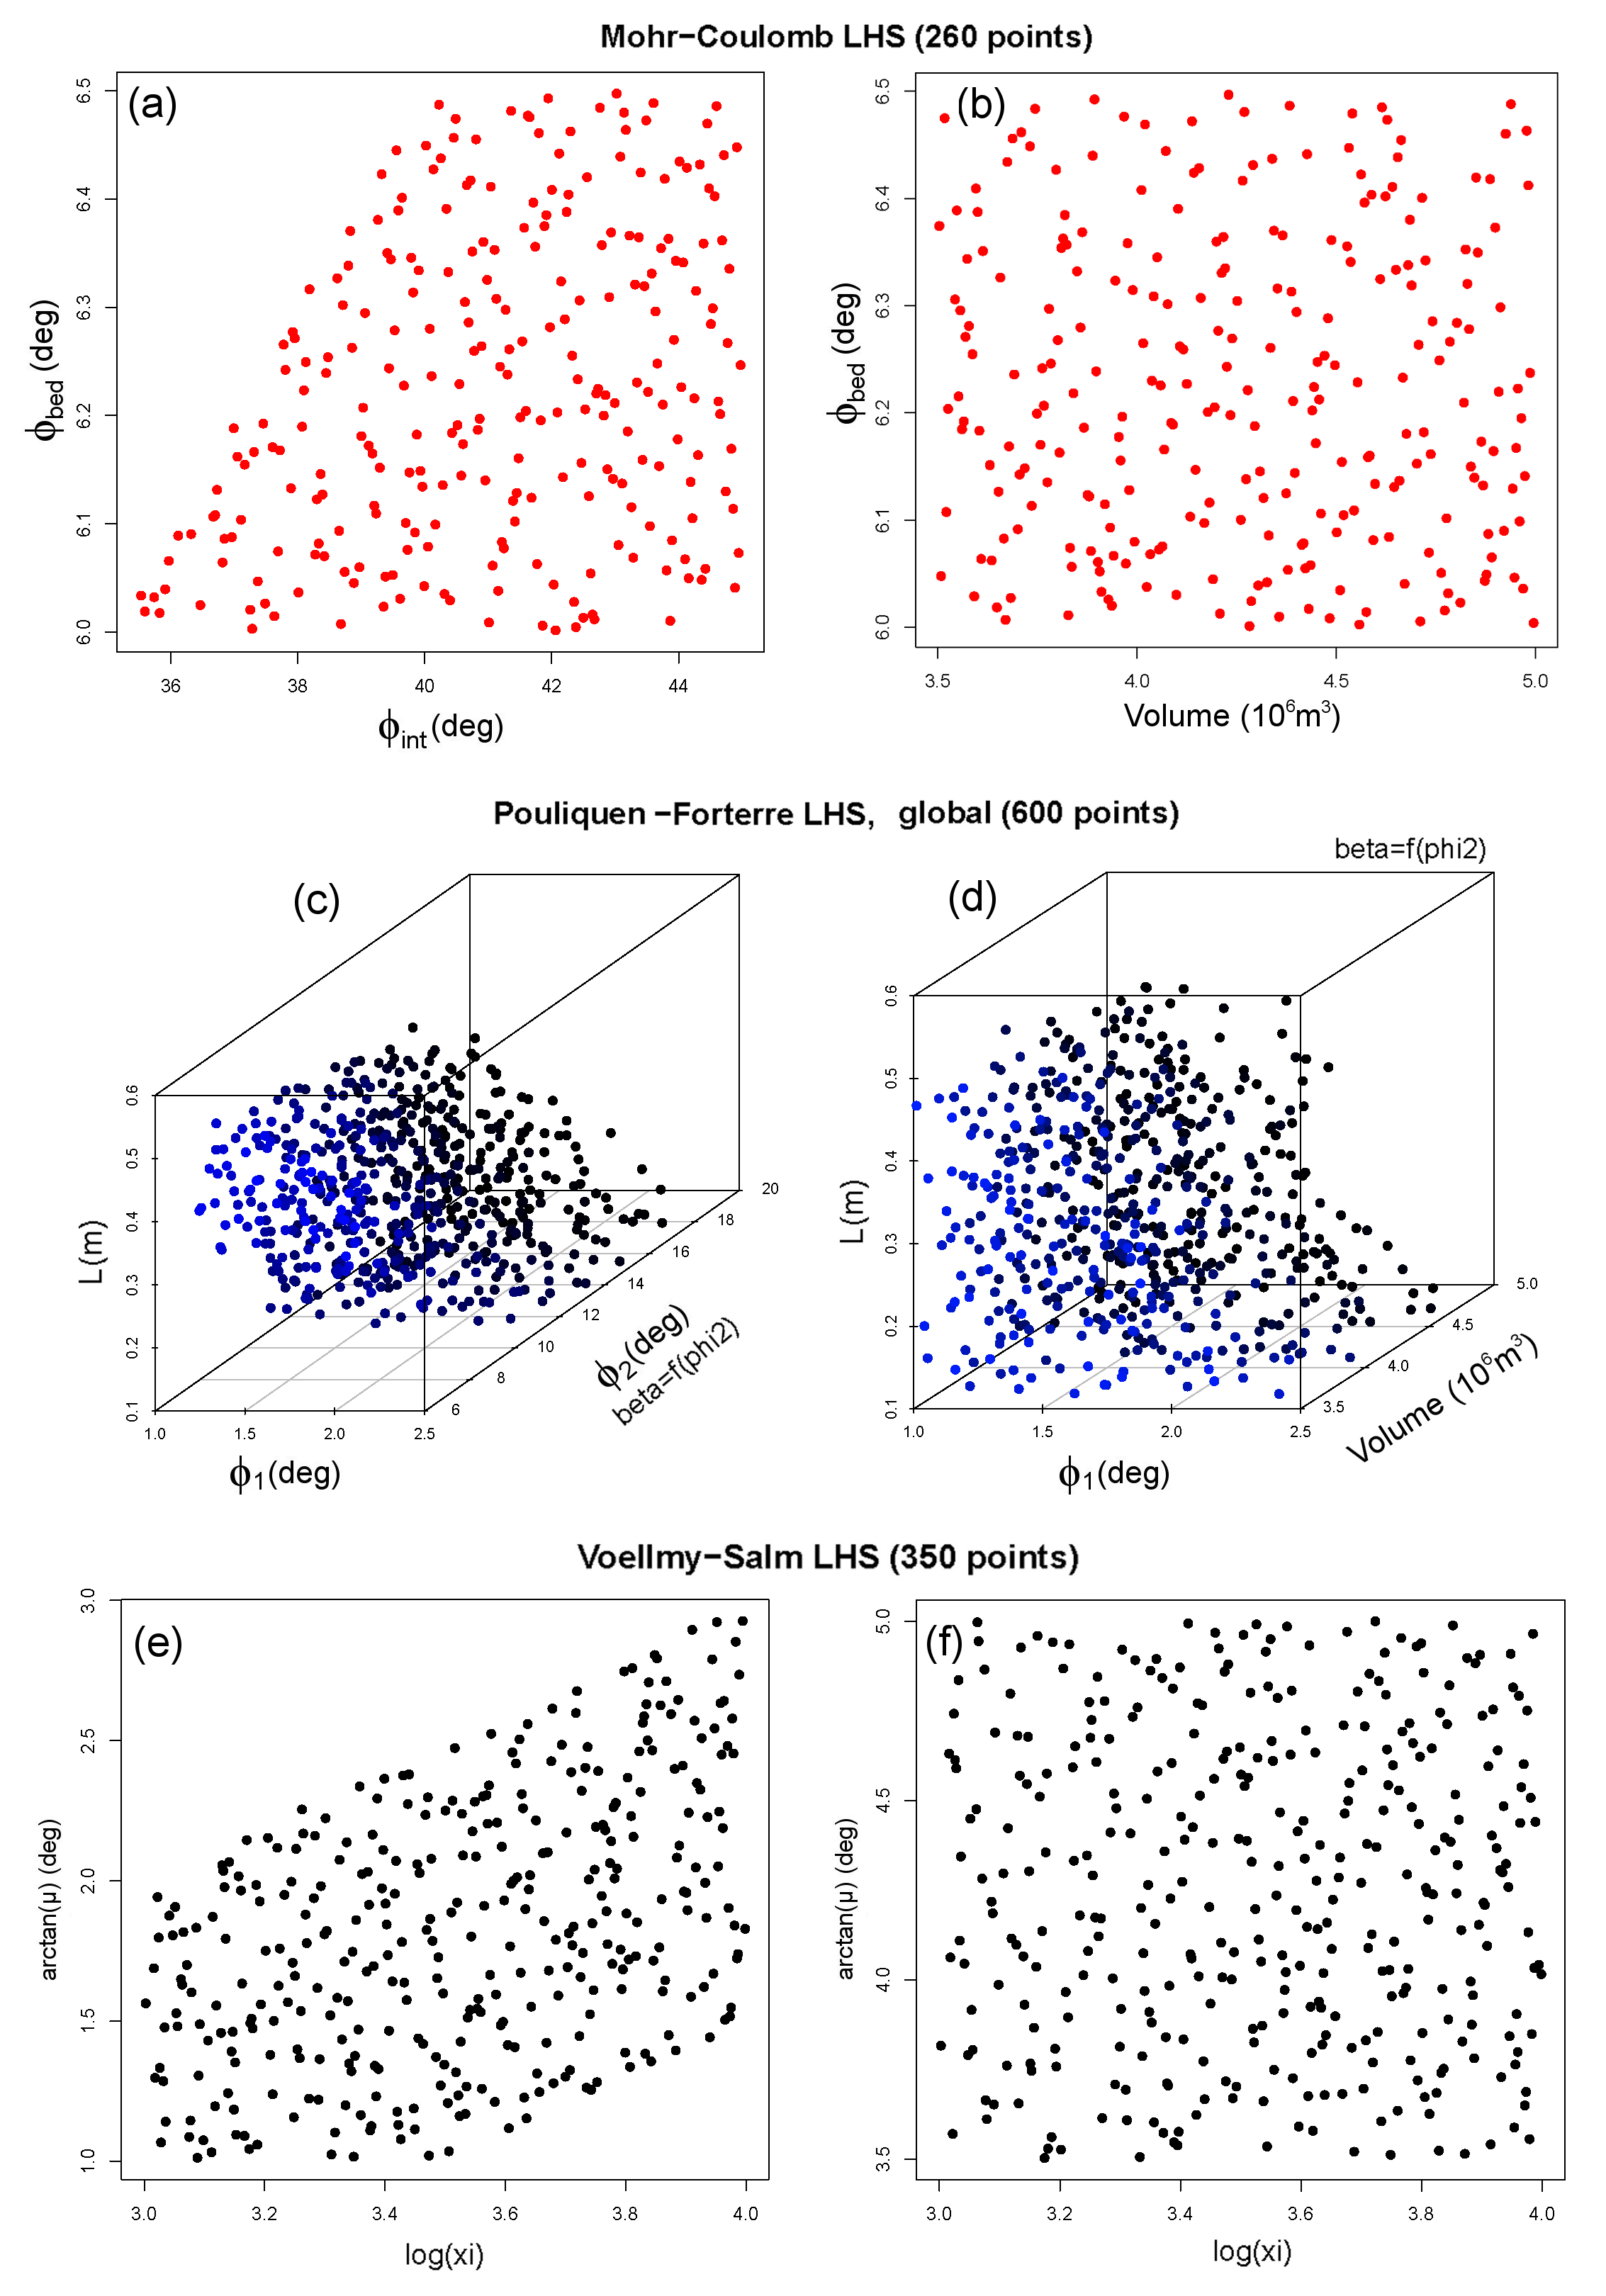
\includegraphics[width=0.87\textwidth]{Fig2.png}
\caption{Overview of the specialized experimental design in (a-b) MC, (c-d) PF, (e-f) VS models. (a-c-e) are projected along the $V$ coordinate, and (b-d-f) along $\phi_{int}$, $\phi_2$ and $\xi$ coordinates, respectively. In (c-d), the color expresses the distance along the third dimension.}
\label{Fig2}
\end{figure}

\subsection{Probability measures and specialized latin hypercube design}
Initially, $\forall j$ we uniformly distribute the measure $P_0^j$ supported on the general input space $(\Omega_0^j, \mathcal F^j_0)$:
\begin{equation}
P_0^j\left(p^j_1,\dots,p^j_{d_j}\right)\sim \bigotimes_{k=1}^{d_j} Unif(a_{k,{M_j}},b_{k,{M_j}}),
\end{equation}
where $(p^j_1,\dots,p^j_{d_j})$ is the parametrization of model $M_j\in\mathcal M$ described above. Latin Hypercube Sampling is performed over $[0,1]^{d_j}$. We enhanced the sampling procedure relying on orthogonal arrays \citep{Owen1992a,Tang1993,Patra2018}. Those dimensionless samples are thus linearly  mapped over the required intervals, providing the general experimental design.

Then, according to the specialized input space definition, we remove the design points which lay outside of the boundary. The new design is distributed according to the probability measure $P^j$: 
\begin{equation}
P^j=P^j_0(\Omega^j)\cdot \iota^j_*(P^j_0)
\end{equation}
push-forward of the inclusion $\iota^j$ of $\Omega^j$ in $\Omega_0^j$, normalized to be a probability. $P^j$ is naturally defined over the $\sigma$-field $\mathcal F^j:=(\iota^j)^{-1}\mathcal F_0^j$.

\begin{figure}[H]
\centering
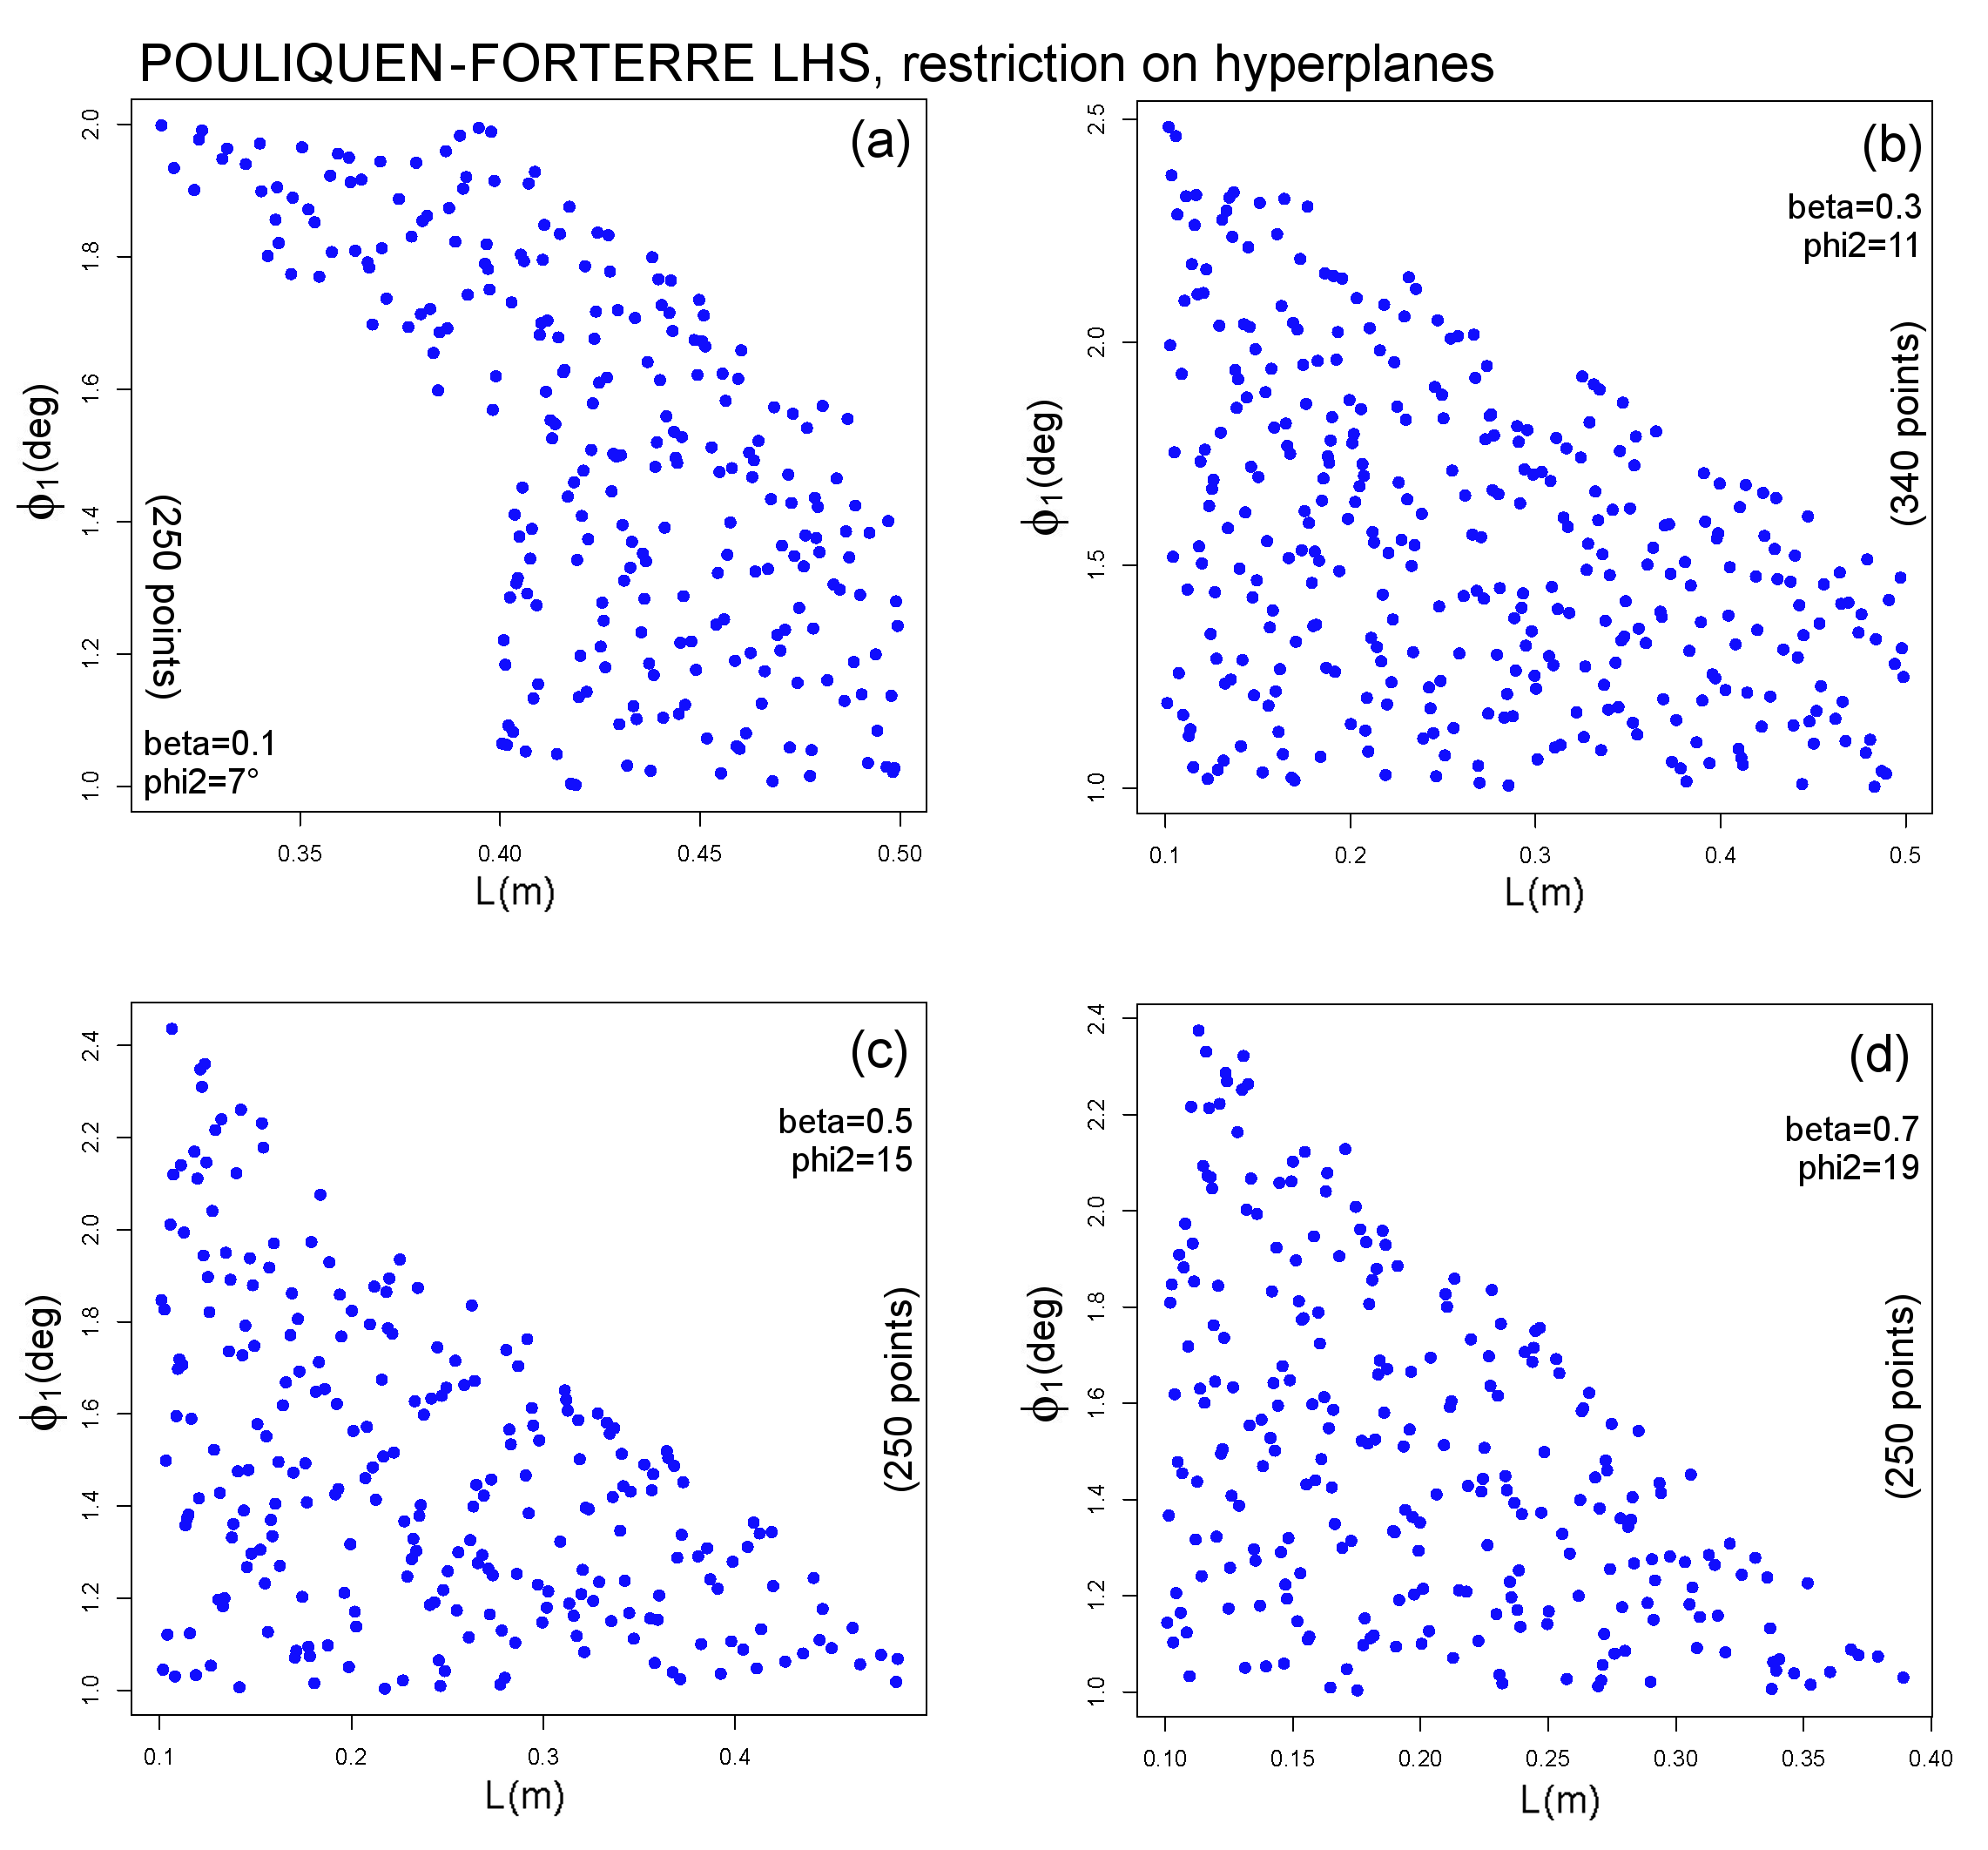
\includegraphics[width=0.87\textwidth]{FigA1.png}
\caption{Overview of modified specialized experimental designs in PF, supported over the four different hyperplanes described in Table 1. All plots are projected along the $V$ coordinate.}
\label{FigA1}
\end{figure}

Figure \ref{Fig2} displays the plot of this specialized experimental design. In PF, the design is immersed in $\mathbb R^4$, and in Figure \ref{FigA1} we show the plot of ancillary experimental designs supported over the four hyperplanes described in Table 1, corresponding to different values of $\phi_2$ and $\beta=f(\phi_2)$.

\section{Statistical analysis of observable outputs and contributing variables}\label{s3}
We devise multiple statistical measures for analyzing the data according to the specialized LHS design described in the previous section. In general, we sample the model inputs in a Monte Carlo simulation, and the output of each sample run is calculated as a function $f(\underline{\textbf x},t)$, where $t$ is the time and $\underline{\textbf x}$ is a spatial element of the computational grid. The family of these functions naturally defines a random variable which expresses the model outputs with respect to the probability distribution $P^j$ over the input space $(\Omega^j, \mathcal F^j)$. This analysis generates tremendous volume of data that we analyzed using statistical methods. The results are summarized by a family of spatial maps and temporal graphs, displaying the expectation of the model outputs and also their 5$^{\mathrm{th}}$ and 95$^{\mathrm{th}}$ percentiles, with respect to $P^j$.

We selected five sites and we gathered detailed results from our simulations in those spatial locations. These are called Site \#1-\#5 and are reported as stars in Figure 1. They all belong to the set of the sixty sections studied in \cite{Saucedo2008}, and the section numbers are also reported. In detail they are placed:
\begin{itemize}
\item\textbf{Site \#1} along the main ravine $\sim$6 km upstream from the Atenquique village;
\item\textbf{Site \#2} in Arroyo Seco tributary, $\sim$2.5 km upstream from the confluence.
\end{itemize}
These are not described in detail, but the corresponding results are included in Supporting Information. We focus our analysis on the other three points, all placed along the main ravine in proximity of Atenquique village. 
\begin{itemize}
\item\textbf{Site \#3} is $\sim$2 km upstream from the village;
\item\textbf{Site \#4} immediately before the village, close to the confluence with Arroyo Seco and Arroyo Pl\'atanos tributaries;
\item\textbf{Site \#5} in the village, $\sim$1 km downstream from the previous site.
\end{itemize}

Among with the locally analyzed outputs, we calculated the local \emph{contributing variables} in the modeling equations. These are quantities in the model evaluation that are usually not observed as outputs from the model. In this case they are the force terms in the conservation laws that characterize the models. They are introduced in \cite{Patra2018} and detailed in Appendix \ref{A-2}.

\subsection{Percentile maps of maximum flow height and kinetic energy}
We report the spatial maps of maximum flow height and kinetic energy.

\begin{figure}[H]
\centering
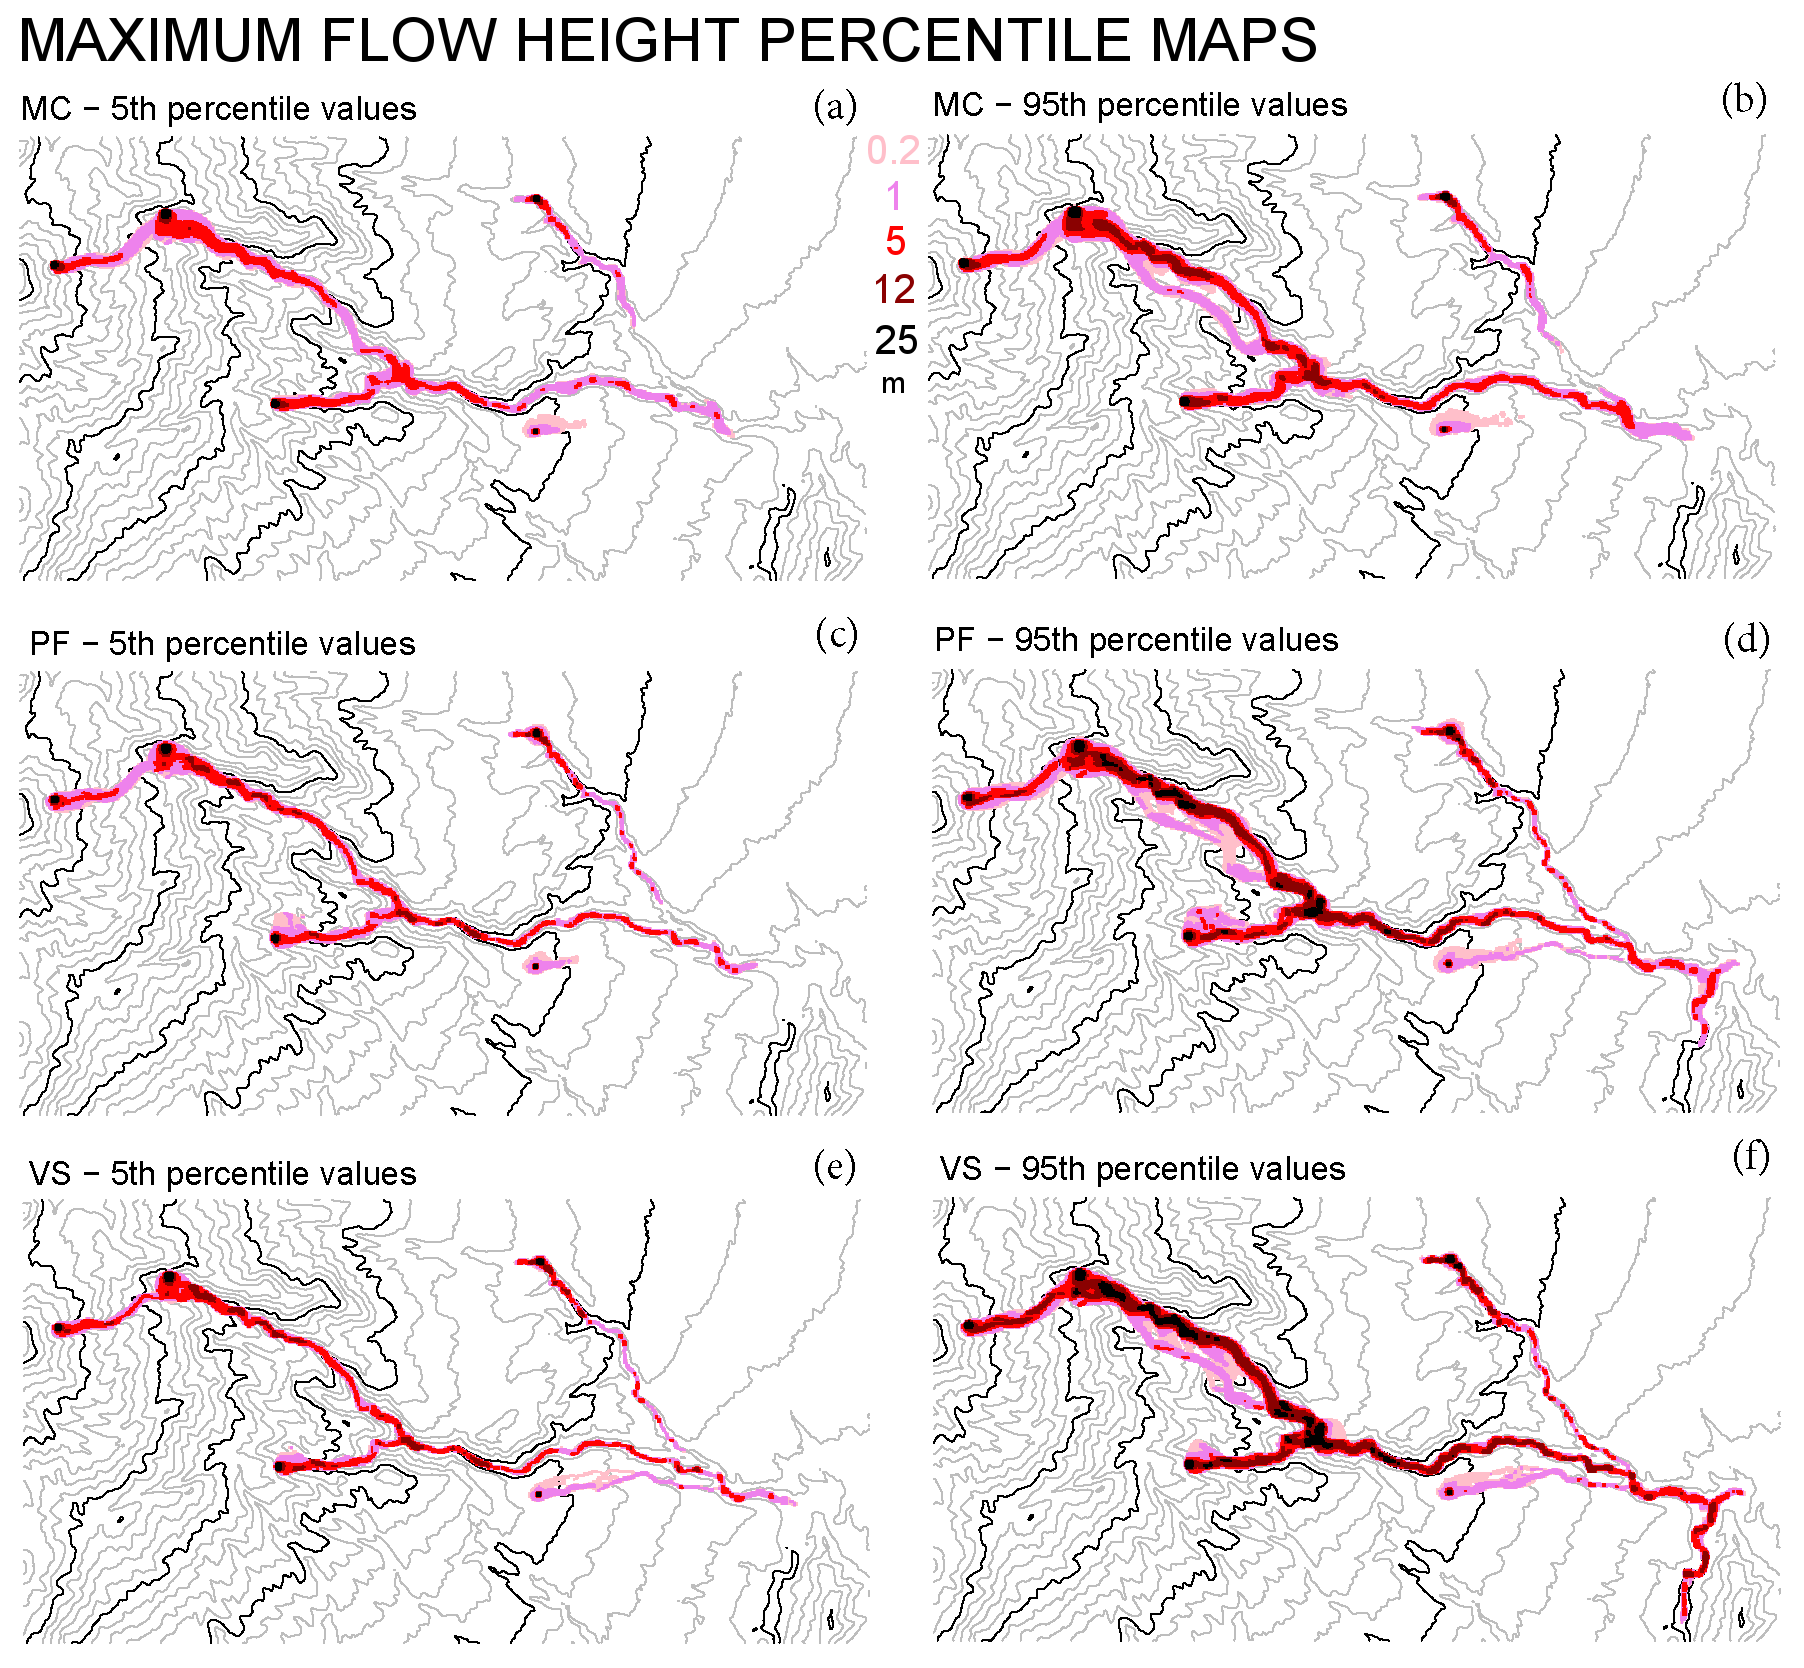
\includegraphics[width=1\textwidth]{Fig3.png}
\caption{Maximum flow height as a function of time}
\label{Fig3}
\end{figure}

\begin{figure}[H]
\centering
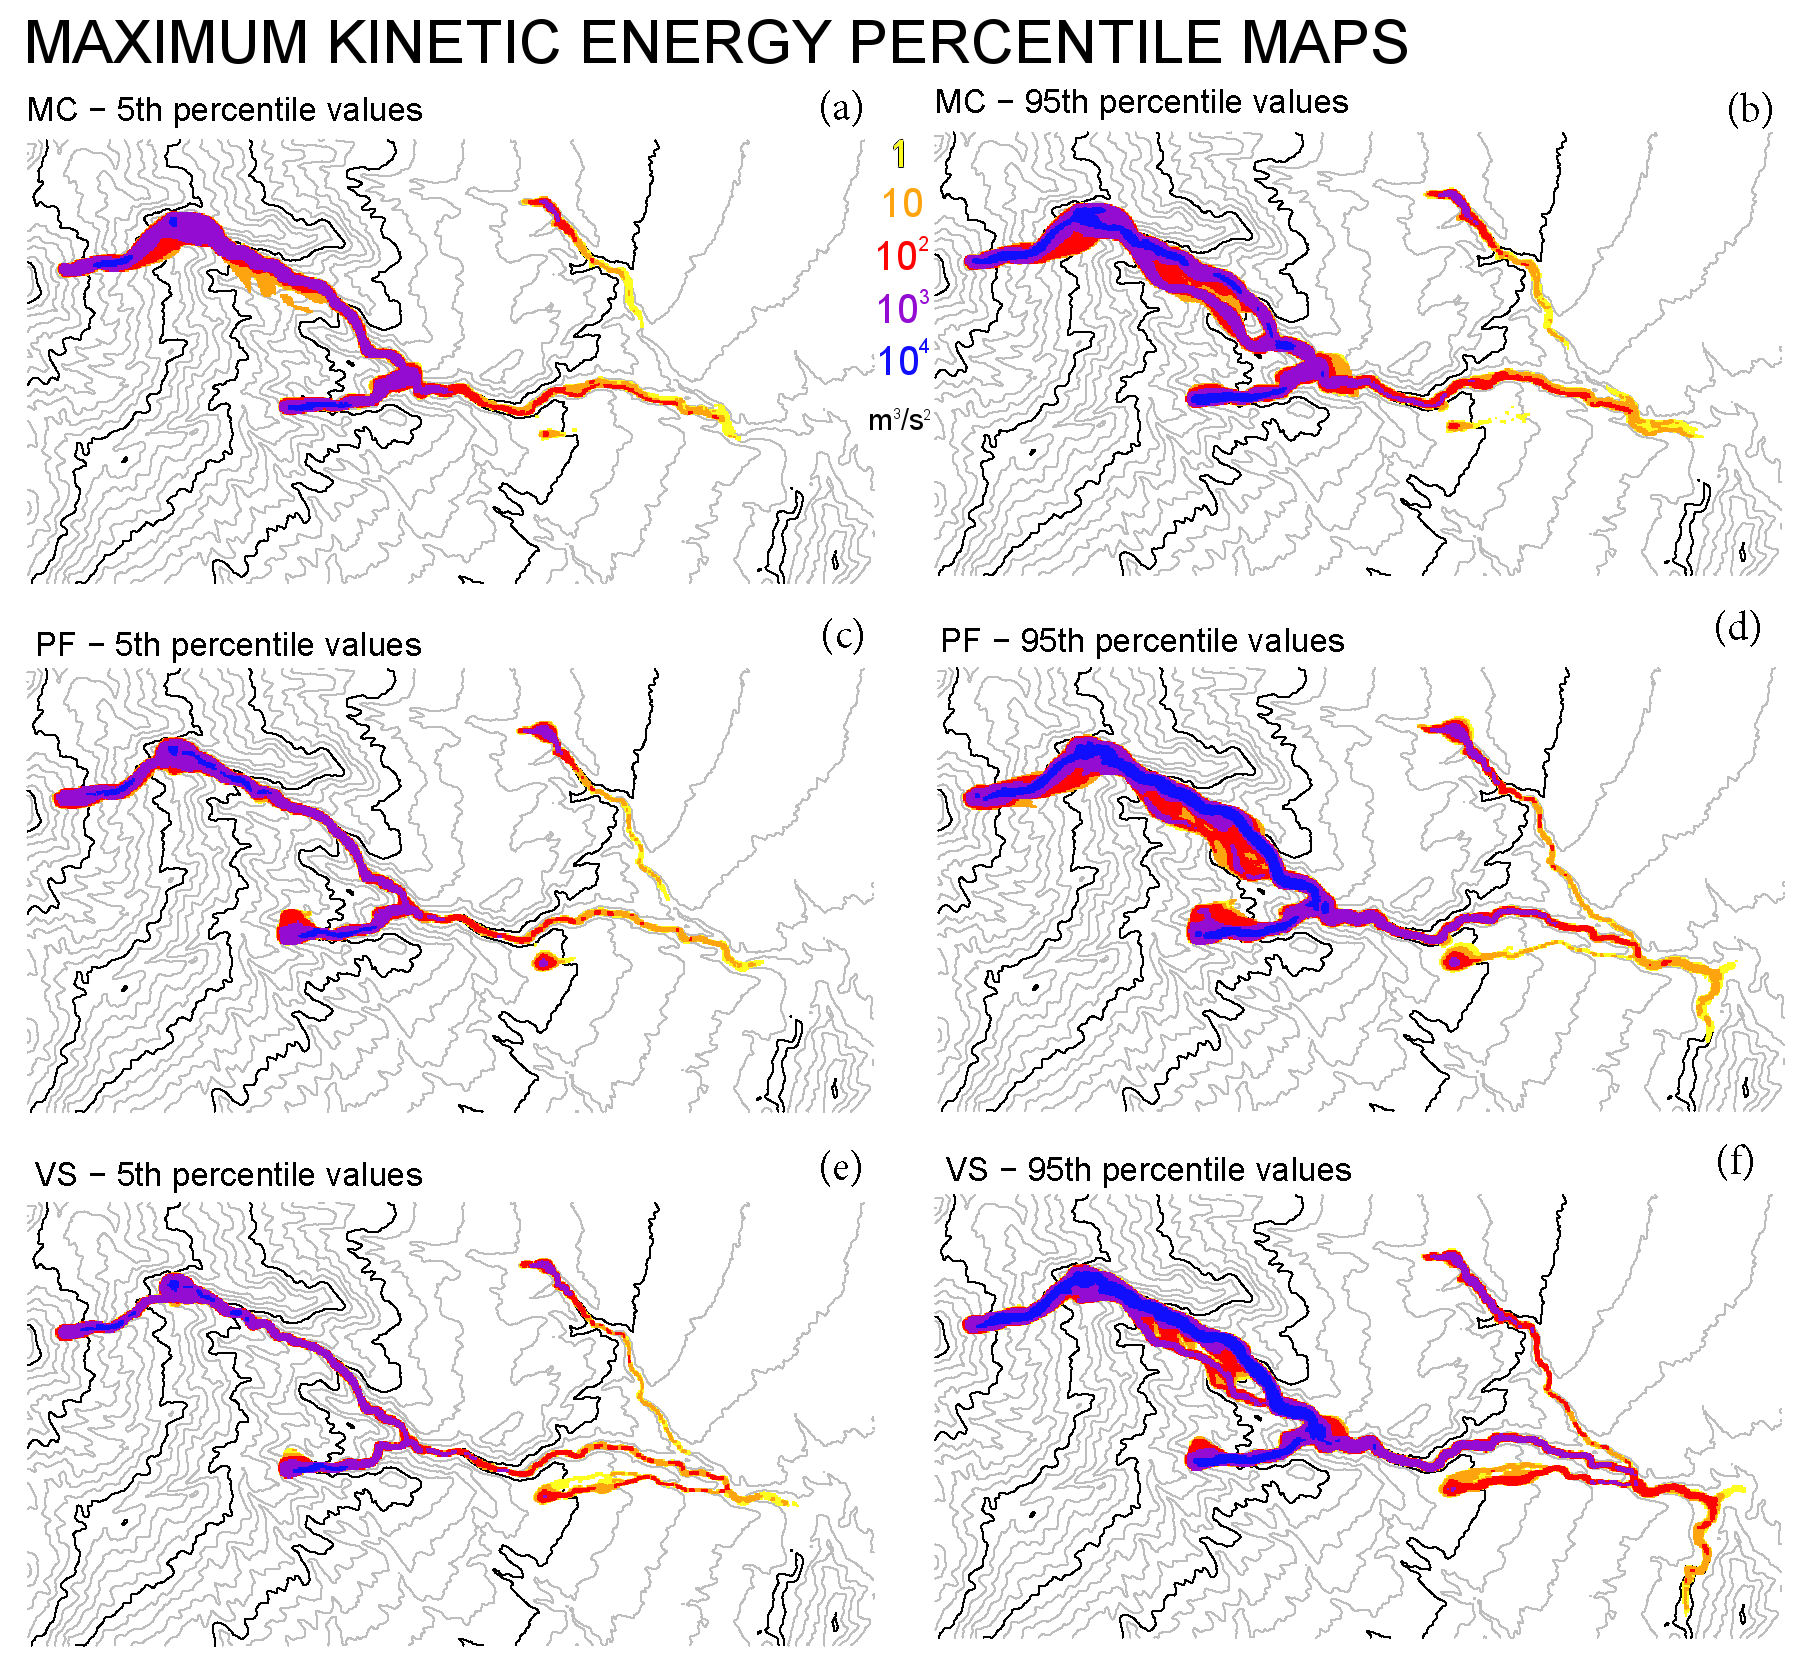
\includegraphics[width=1\textwidth]{Fig4.png}
\caption{...}
\label{Fig4}
\end{figure}

\subsection{Observable outputs and contributing variables}
We locally analyze flow height and speed, and contribution variables in three different locations (sites \#3,\#4, \#5).

\begin{figure}[H]
\centering
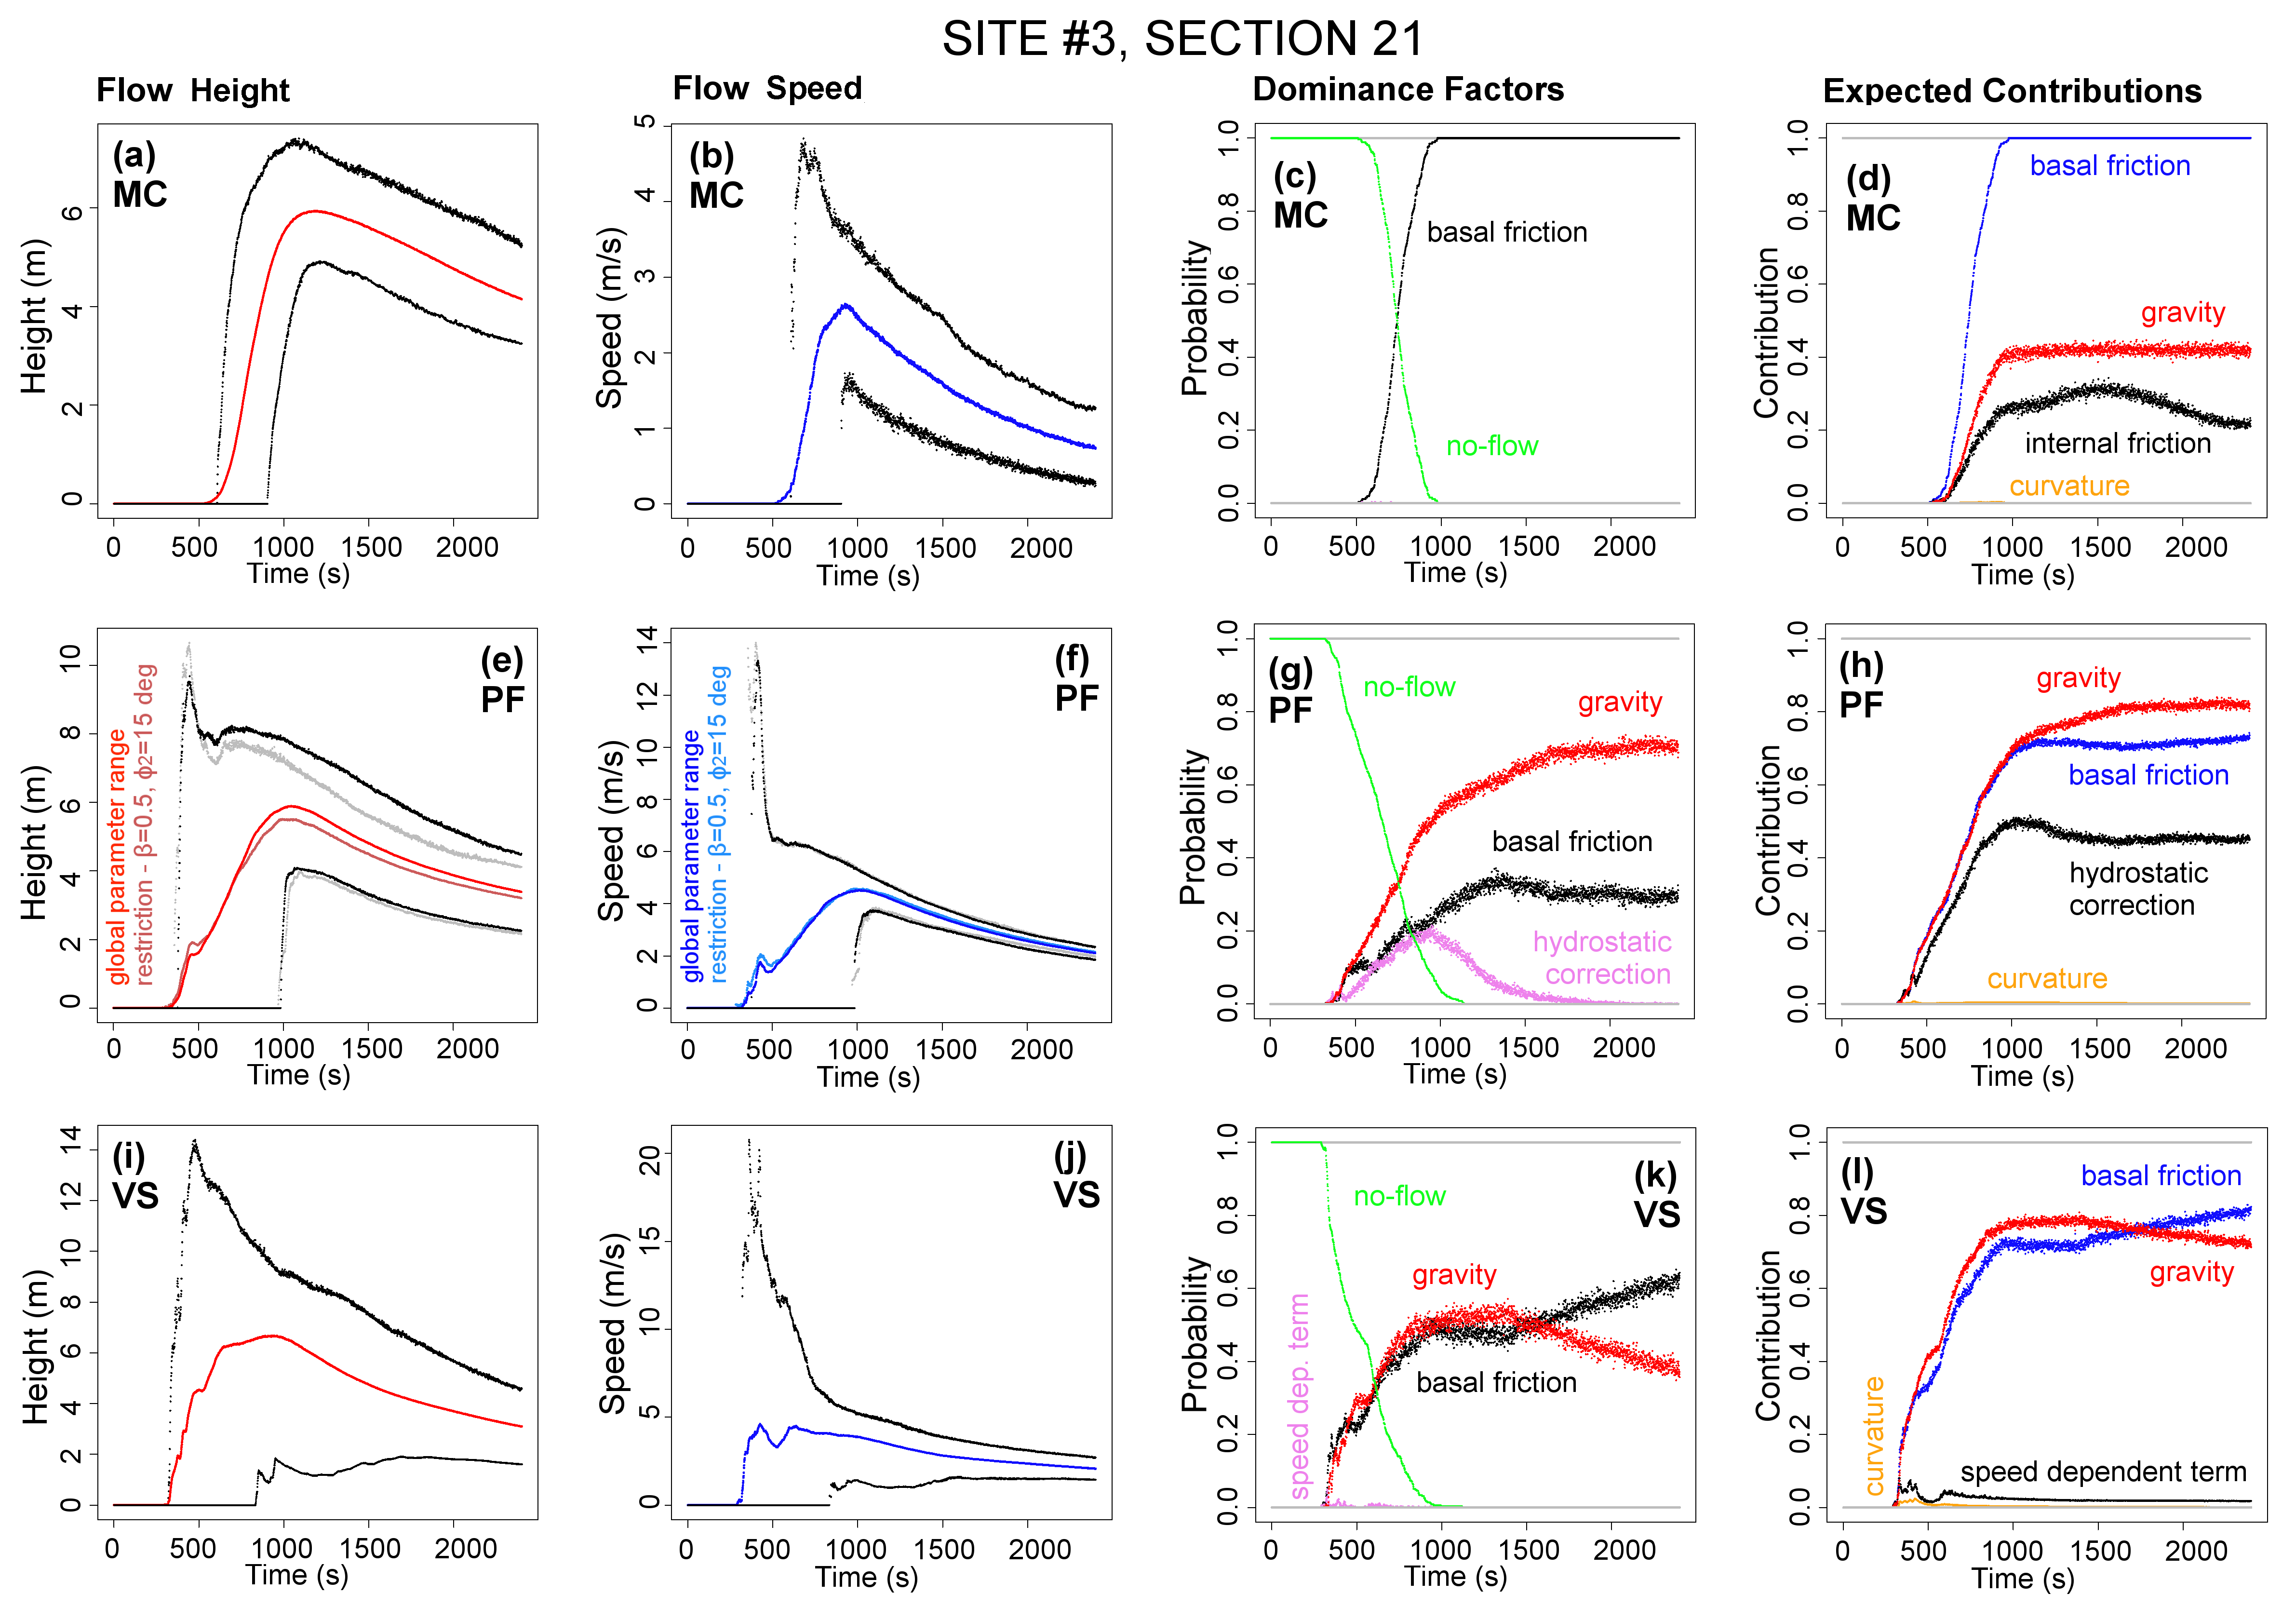
\includegraphics[width=1\textwidth]{Fig5.png}
\caption{...}
\label{Fig5}
\end{figure}

\begin{figure}[H]
\centering
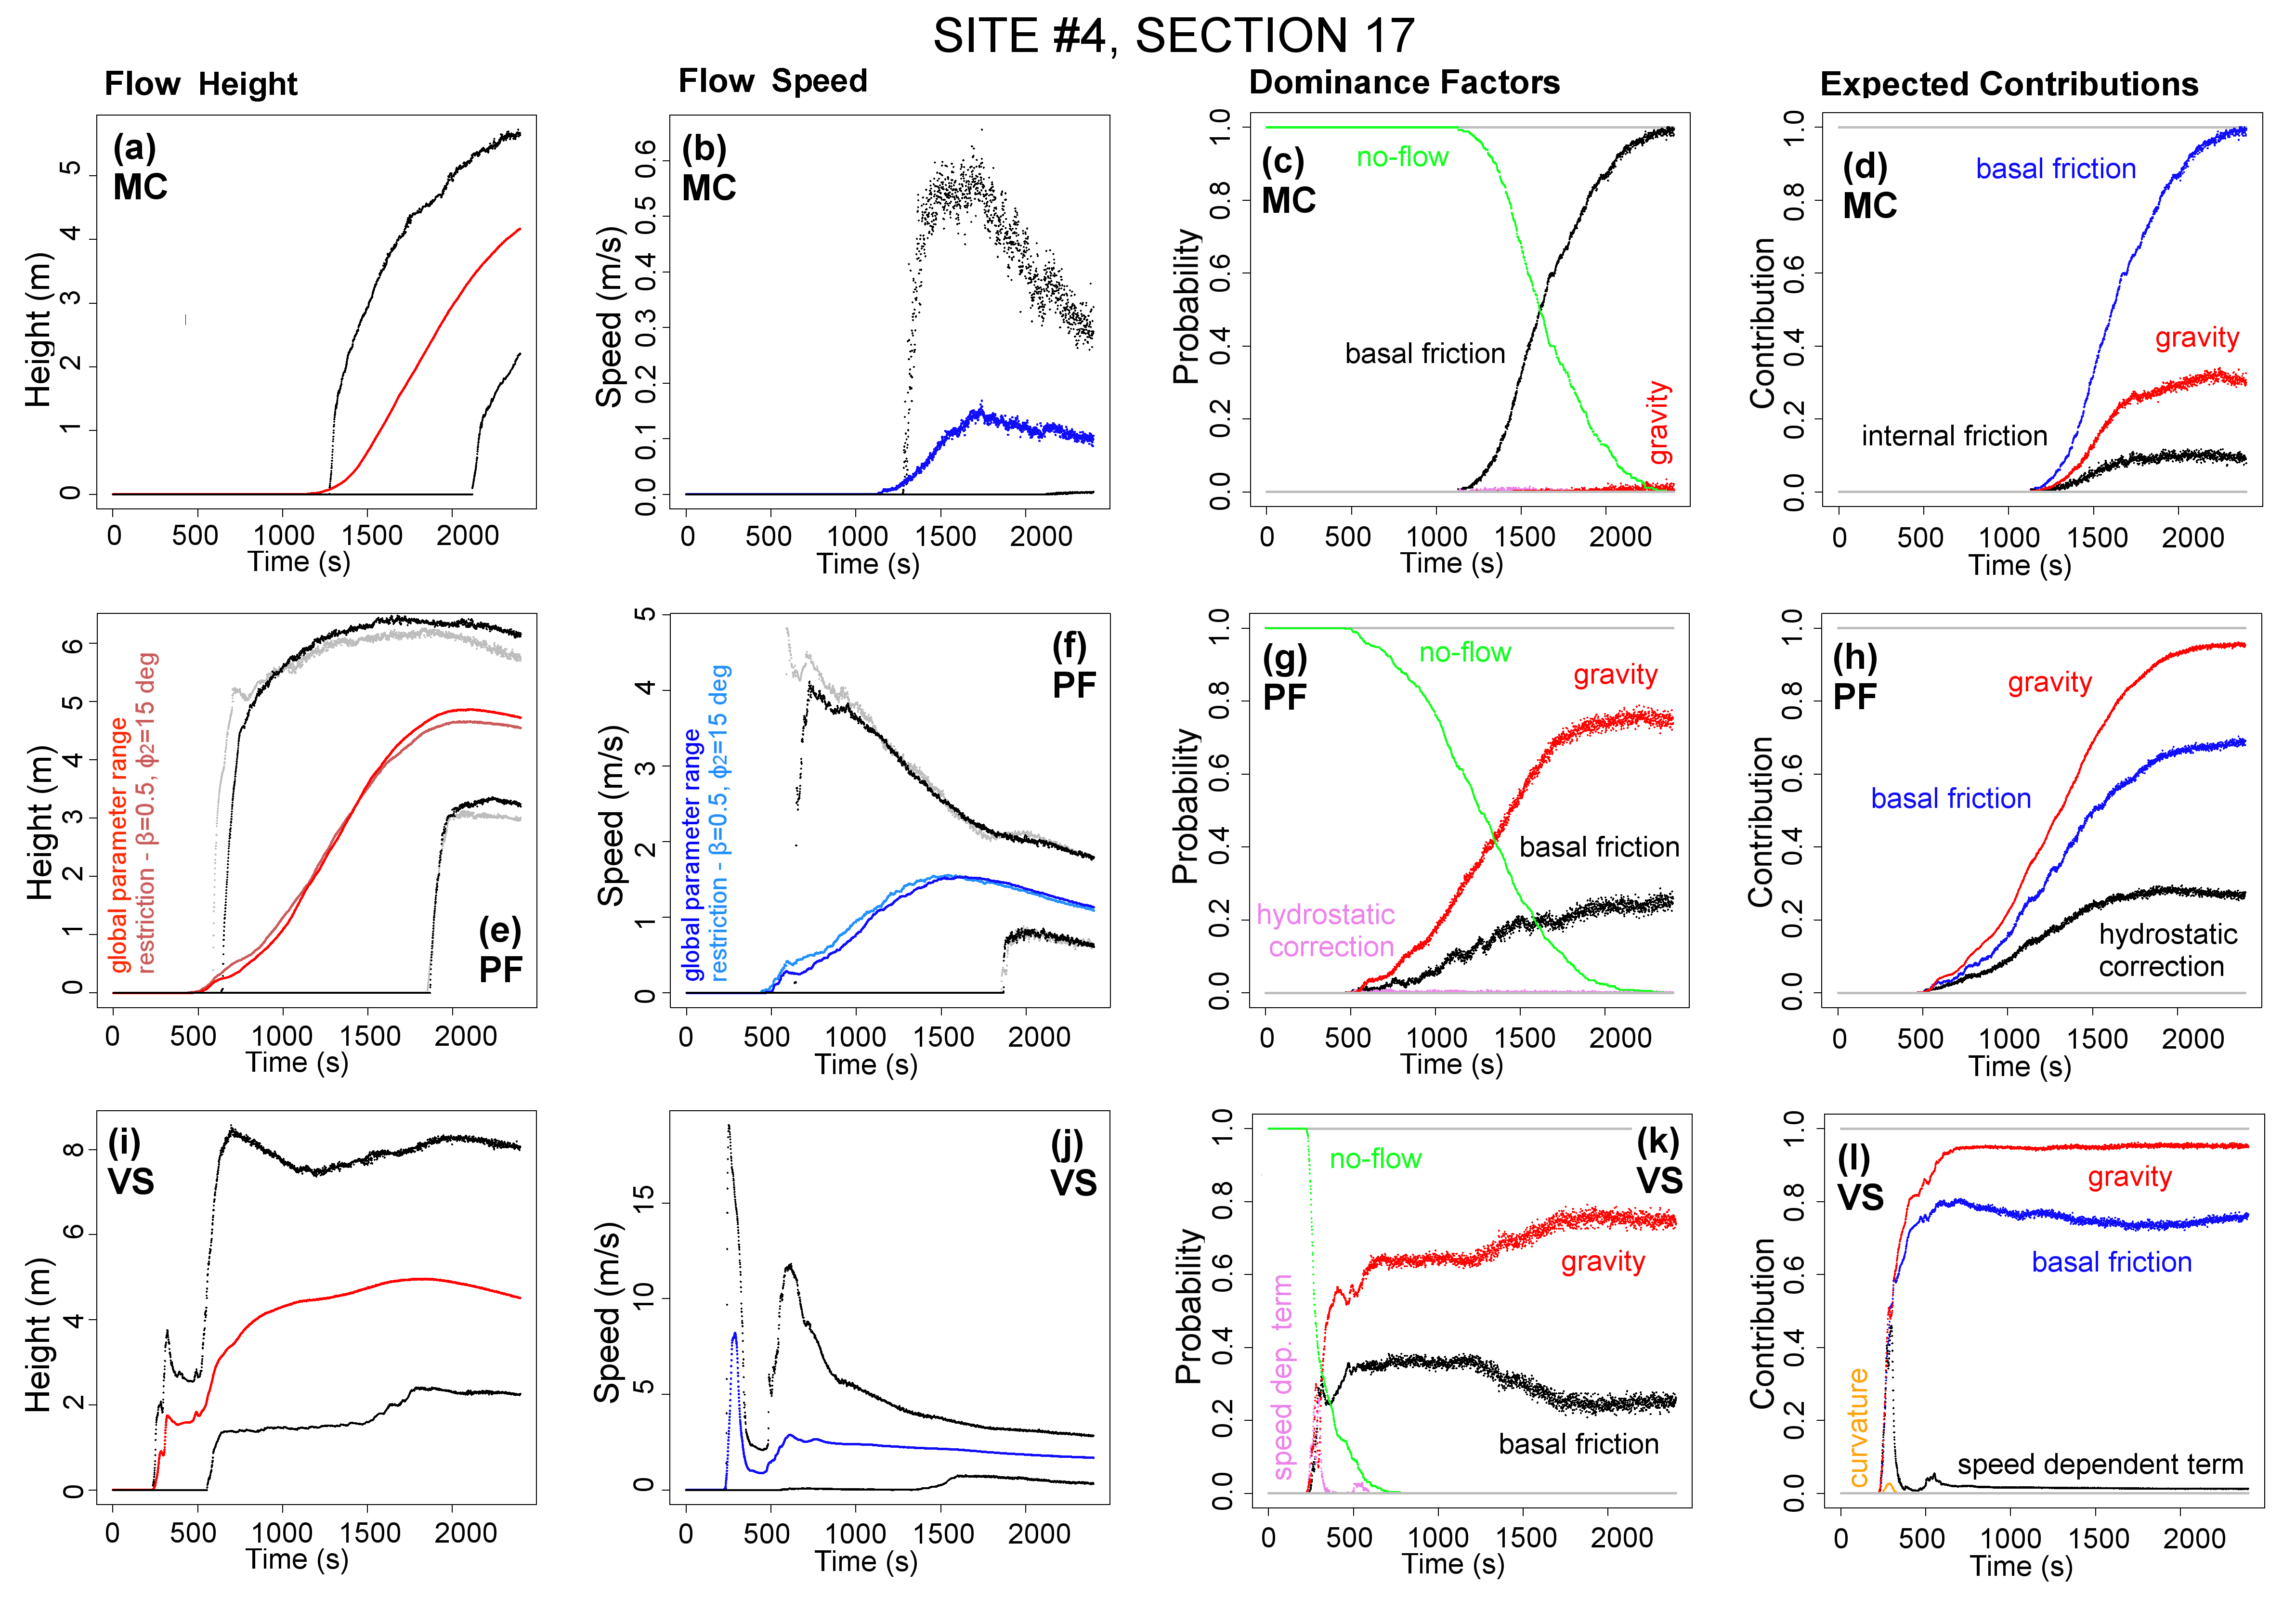
\includegraphics[width=1\textwidth]{Fig6.png}
\caption{...}
\label{Fig6}
\end{figure}

\begin{figure}[H]
\centering
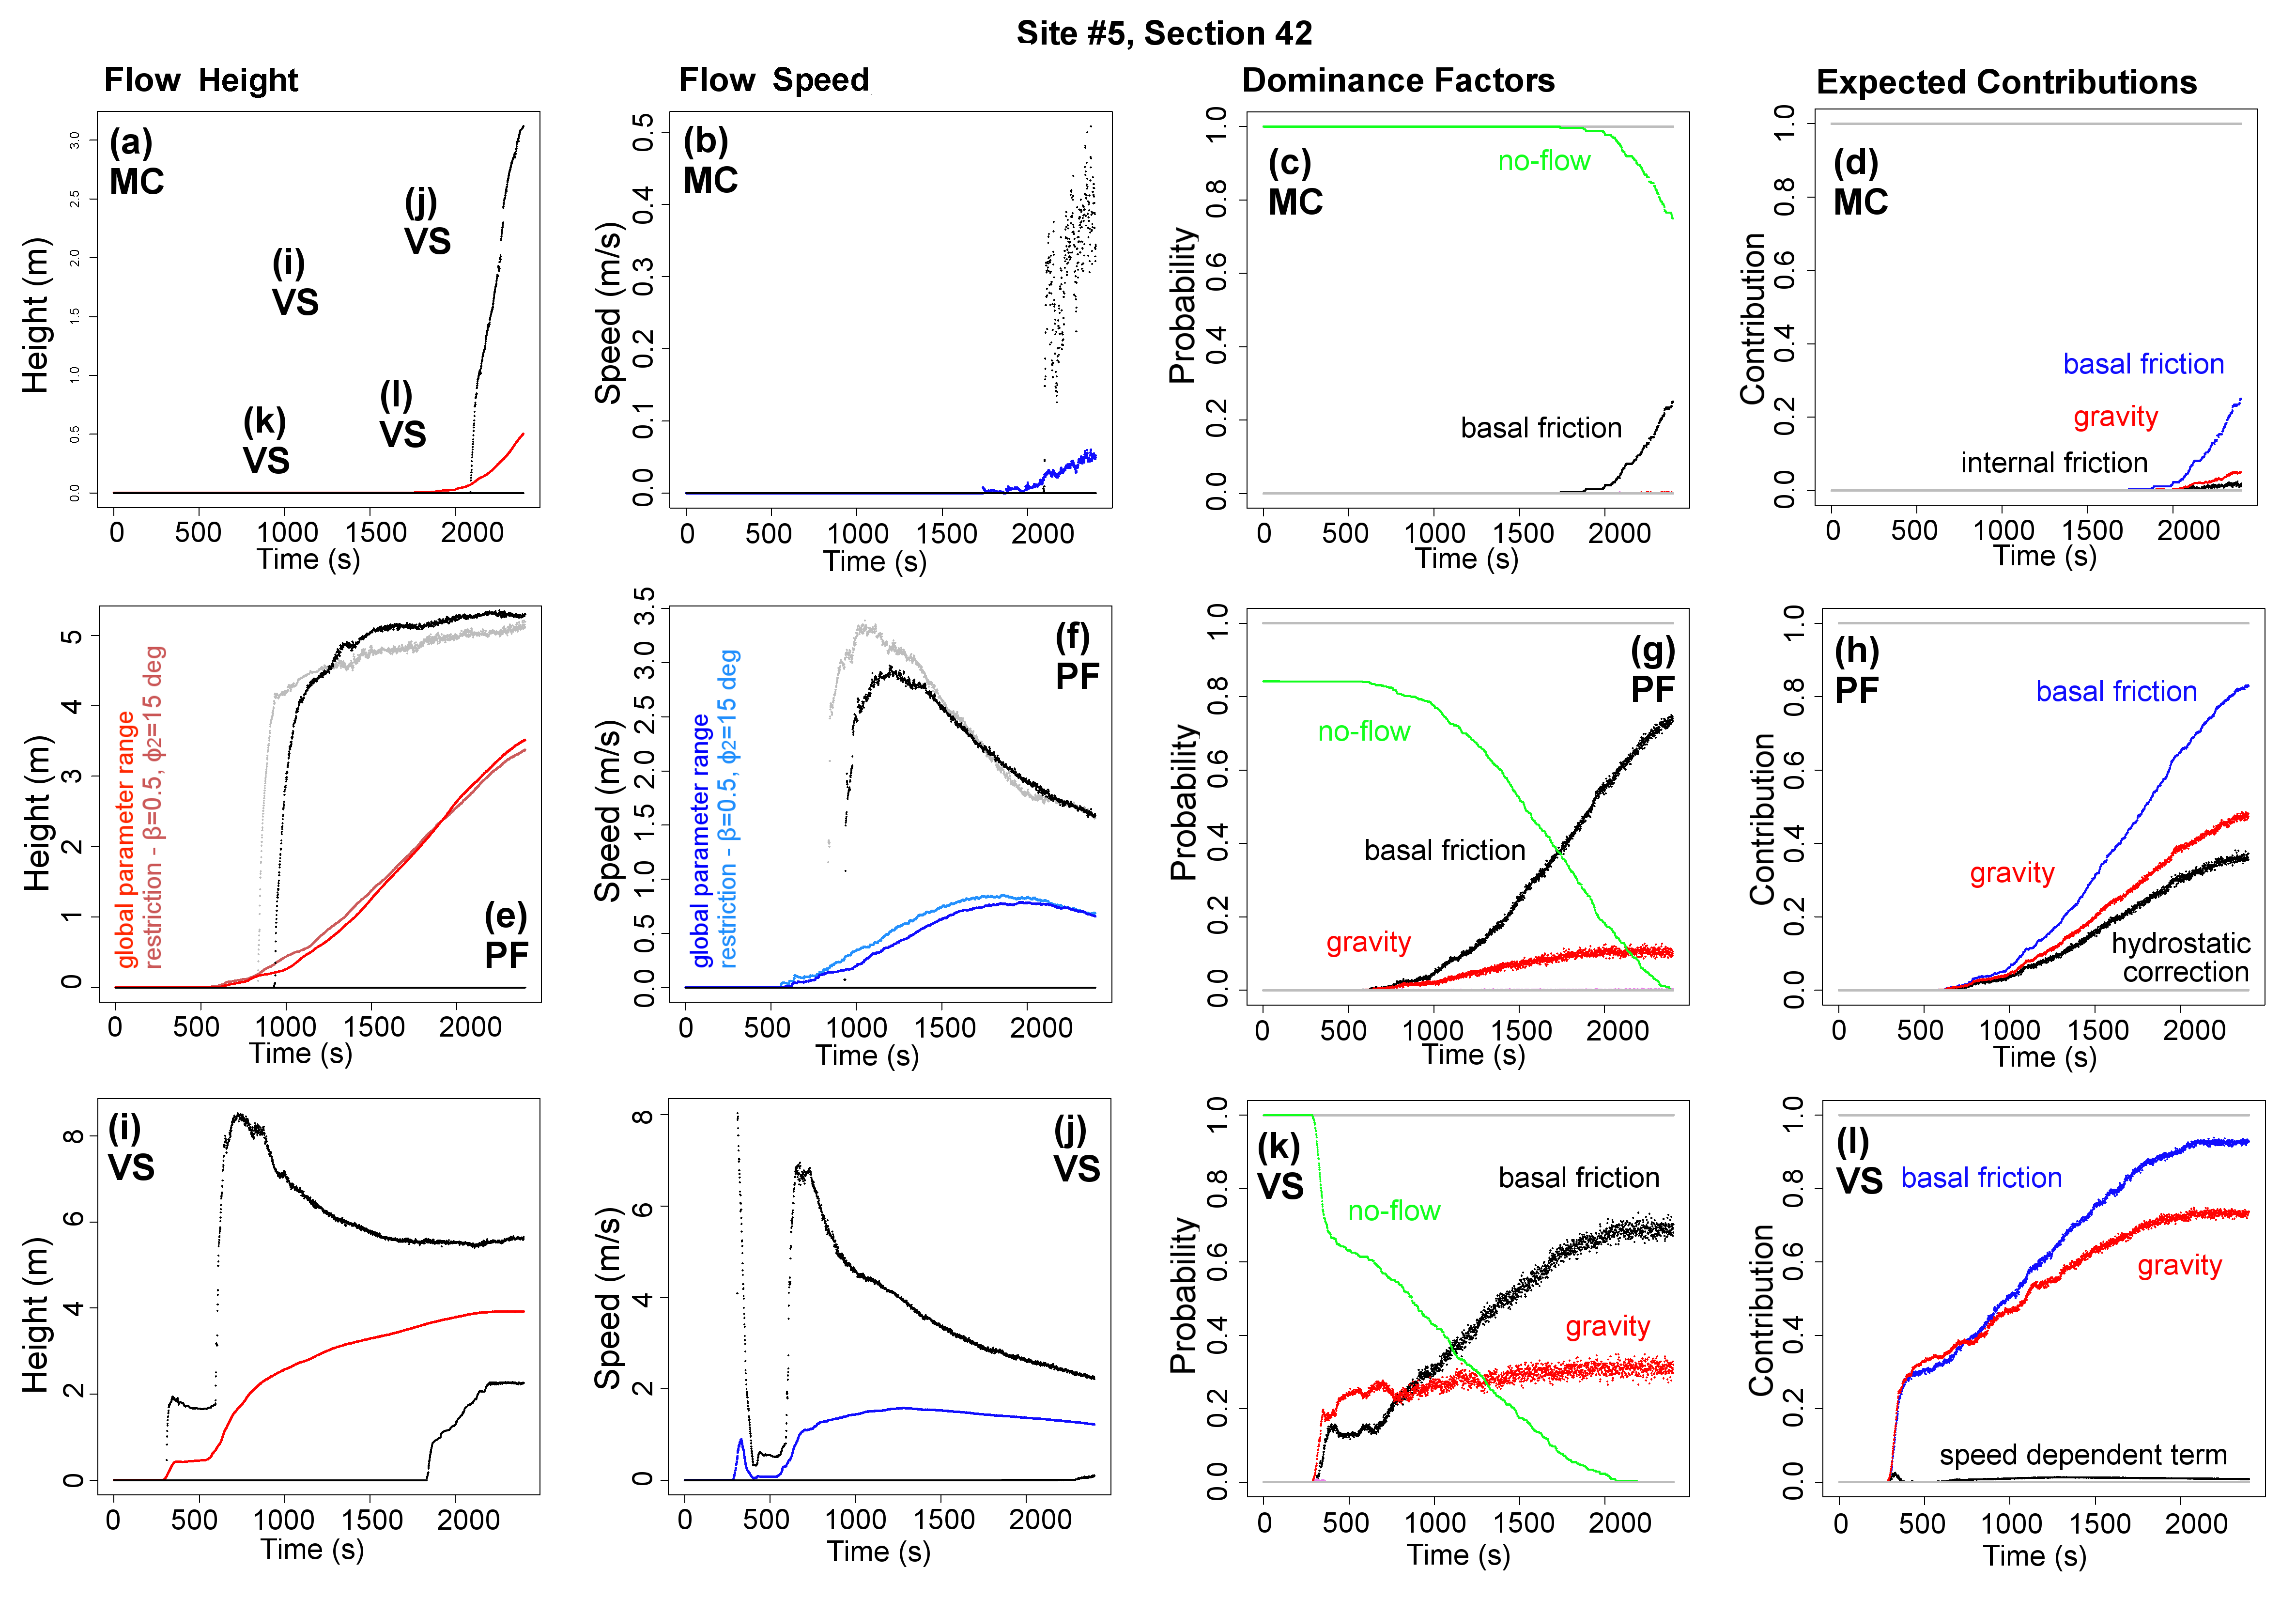
\includegraphics[width=1\textwidth]{Fig7.png}
\caption{...}
\label{Fig7}
\end{figure}

\section{The likelihood of uncertain data}\label{s4}

\begin{figure}[H]
\centering
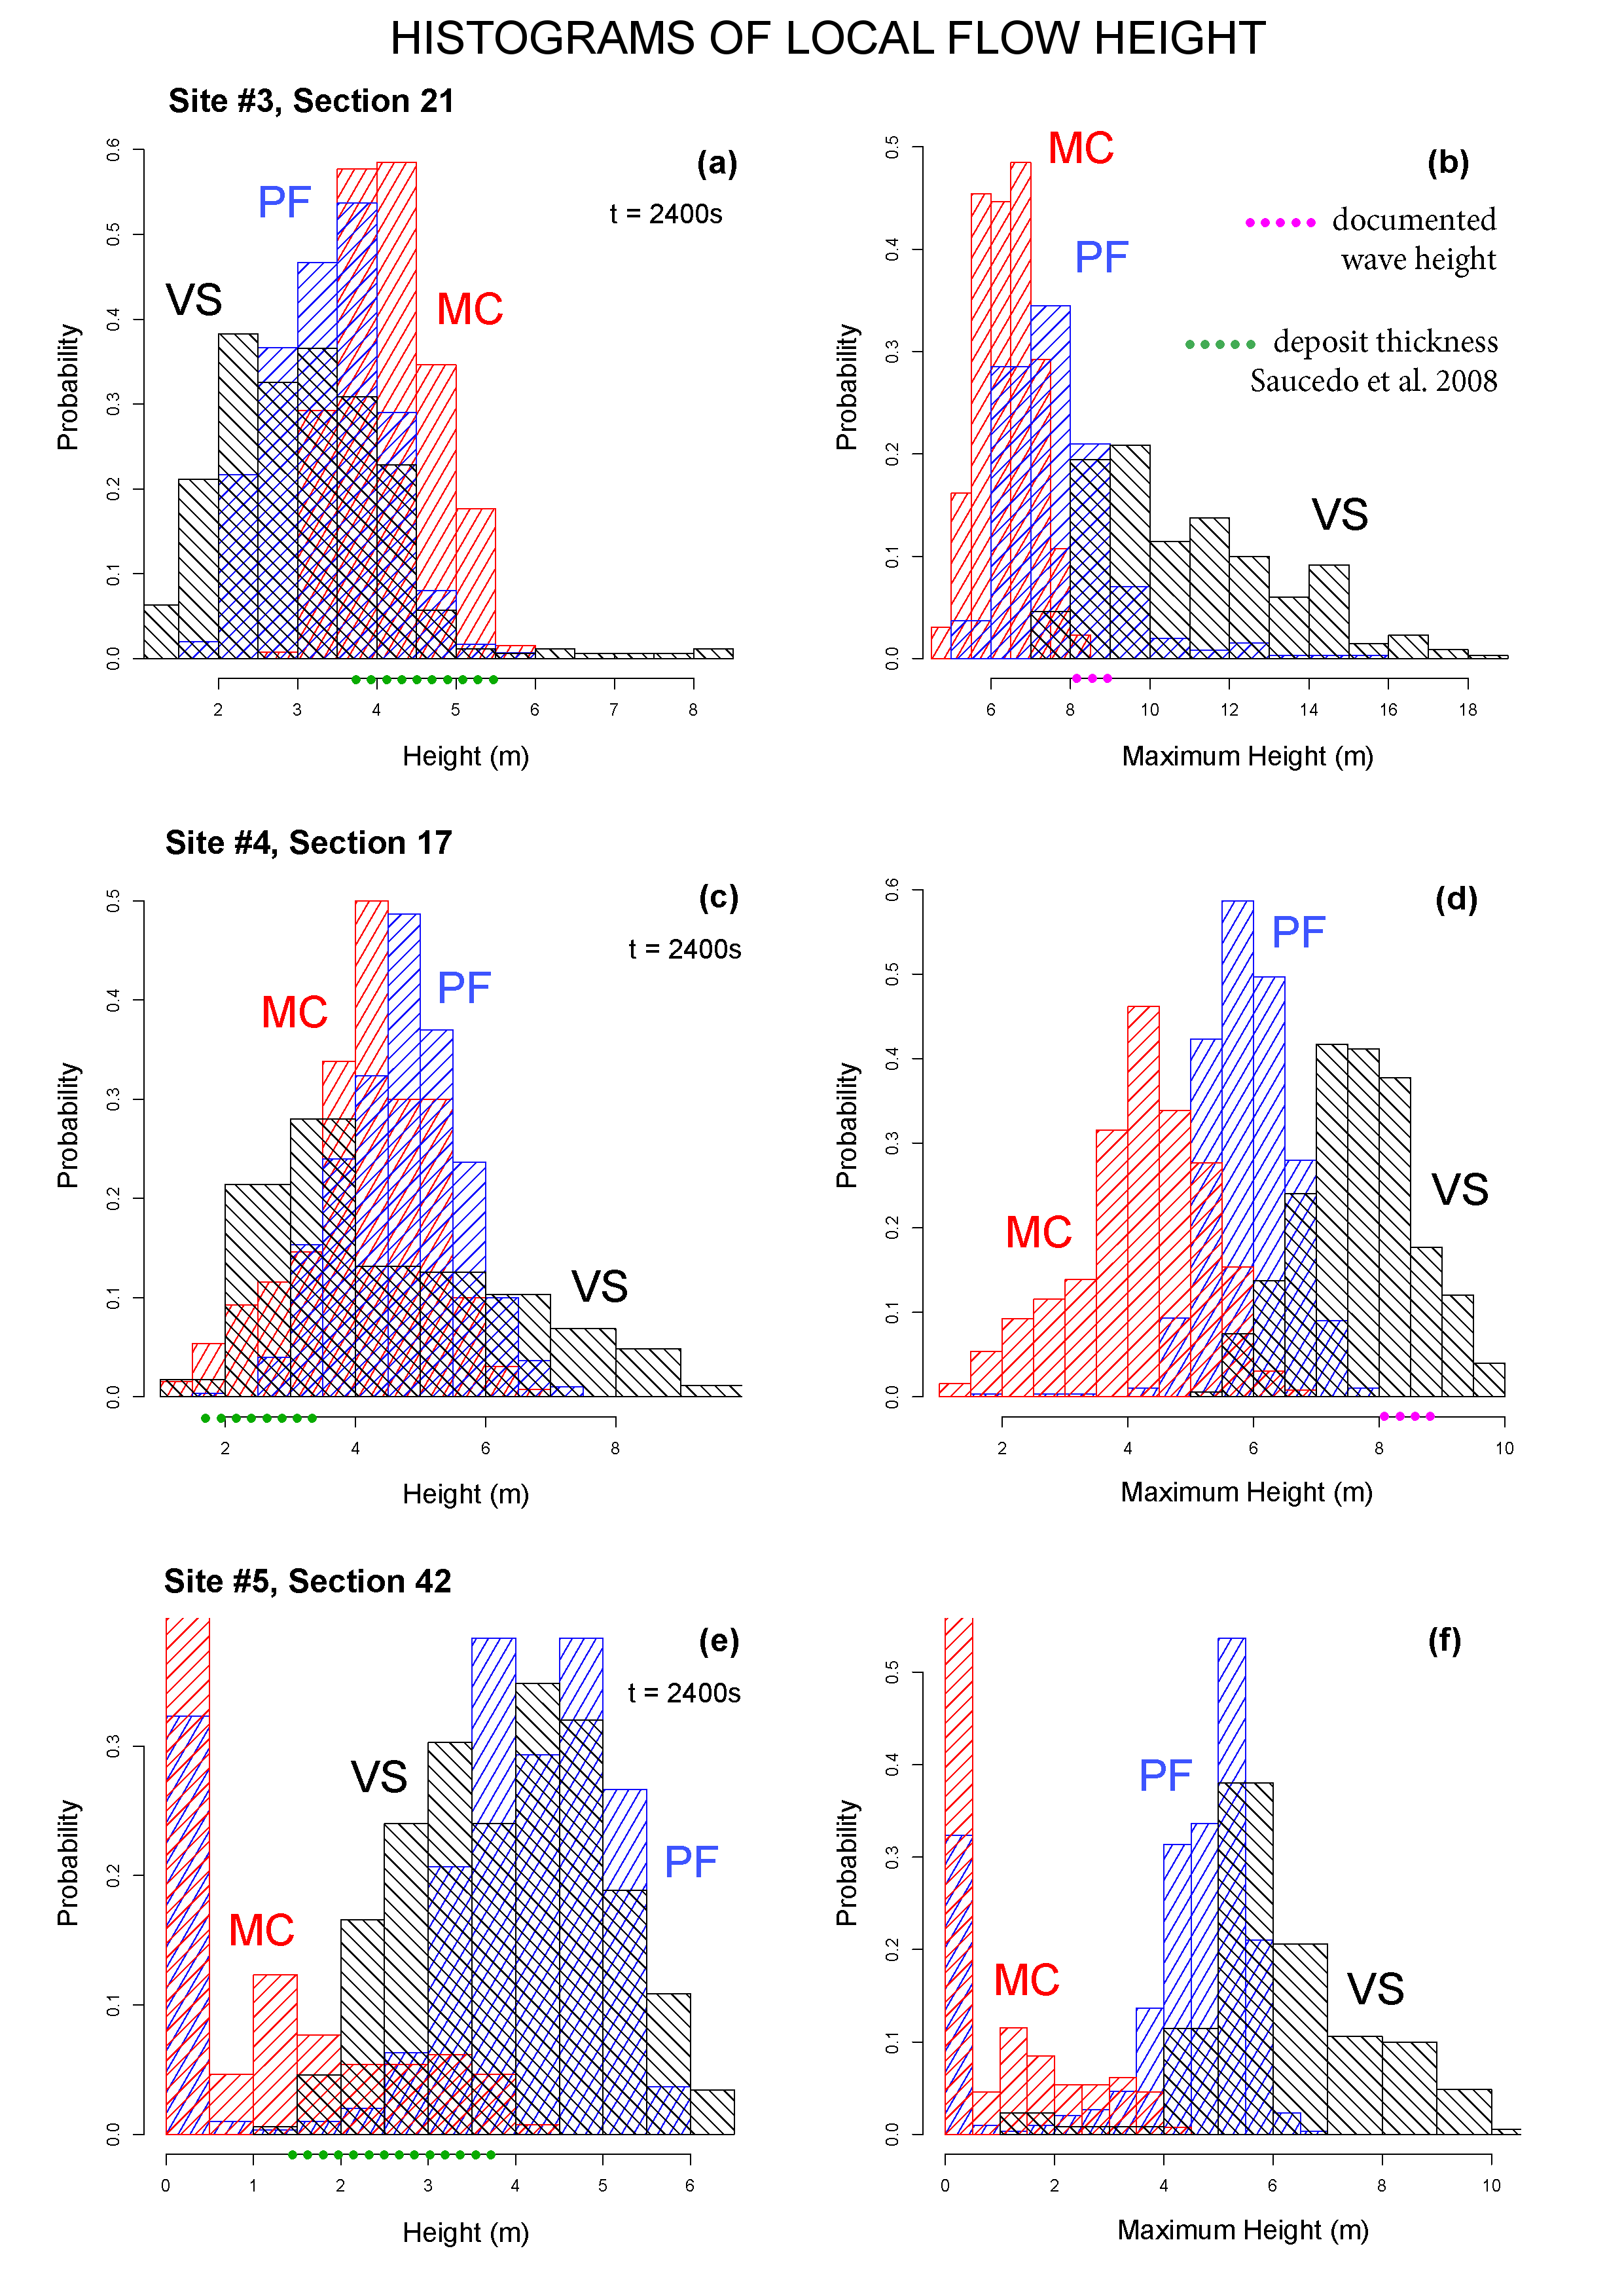
\includegraphics[width=0.8\textwidth]{Fig8.png}
\caption{...}
\label{Fig8}
\end{figure}

\begin{figure}[H]
\centering
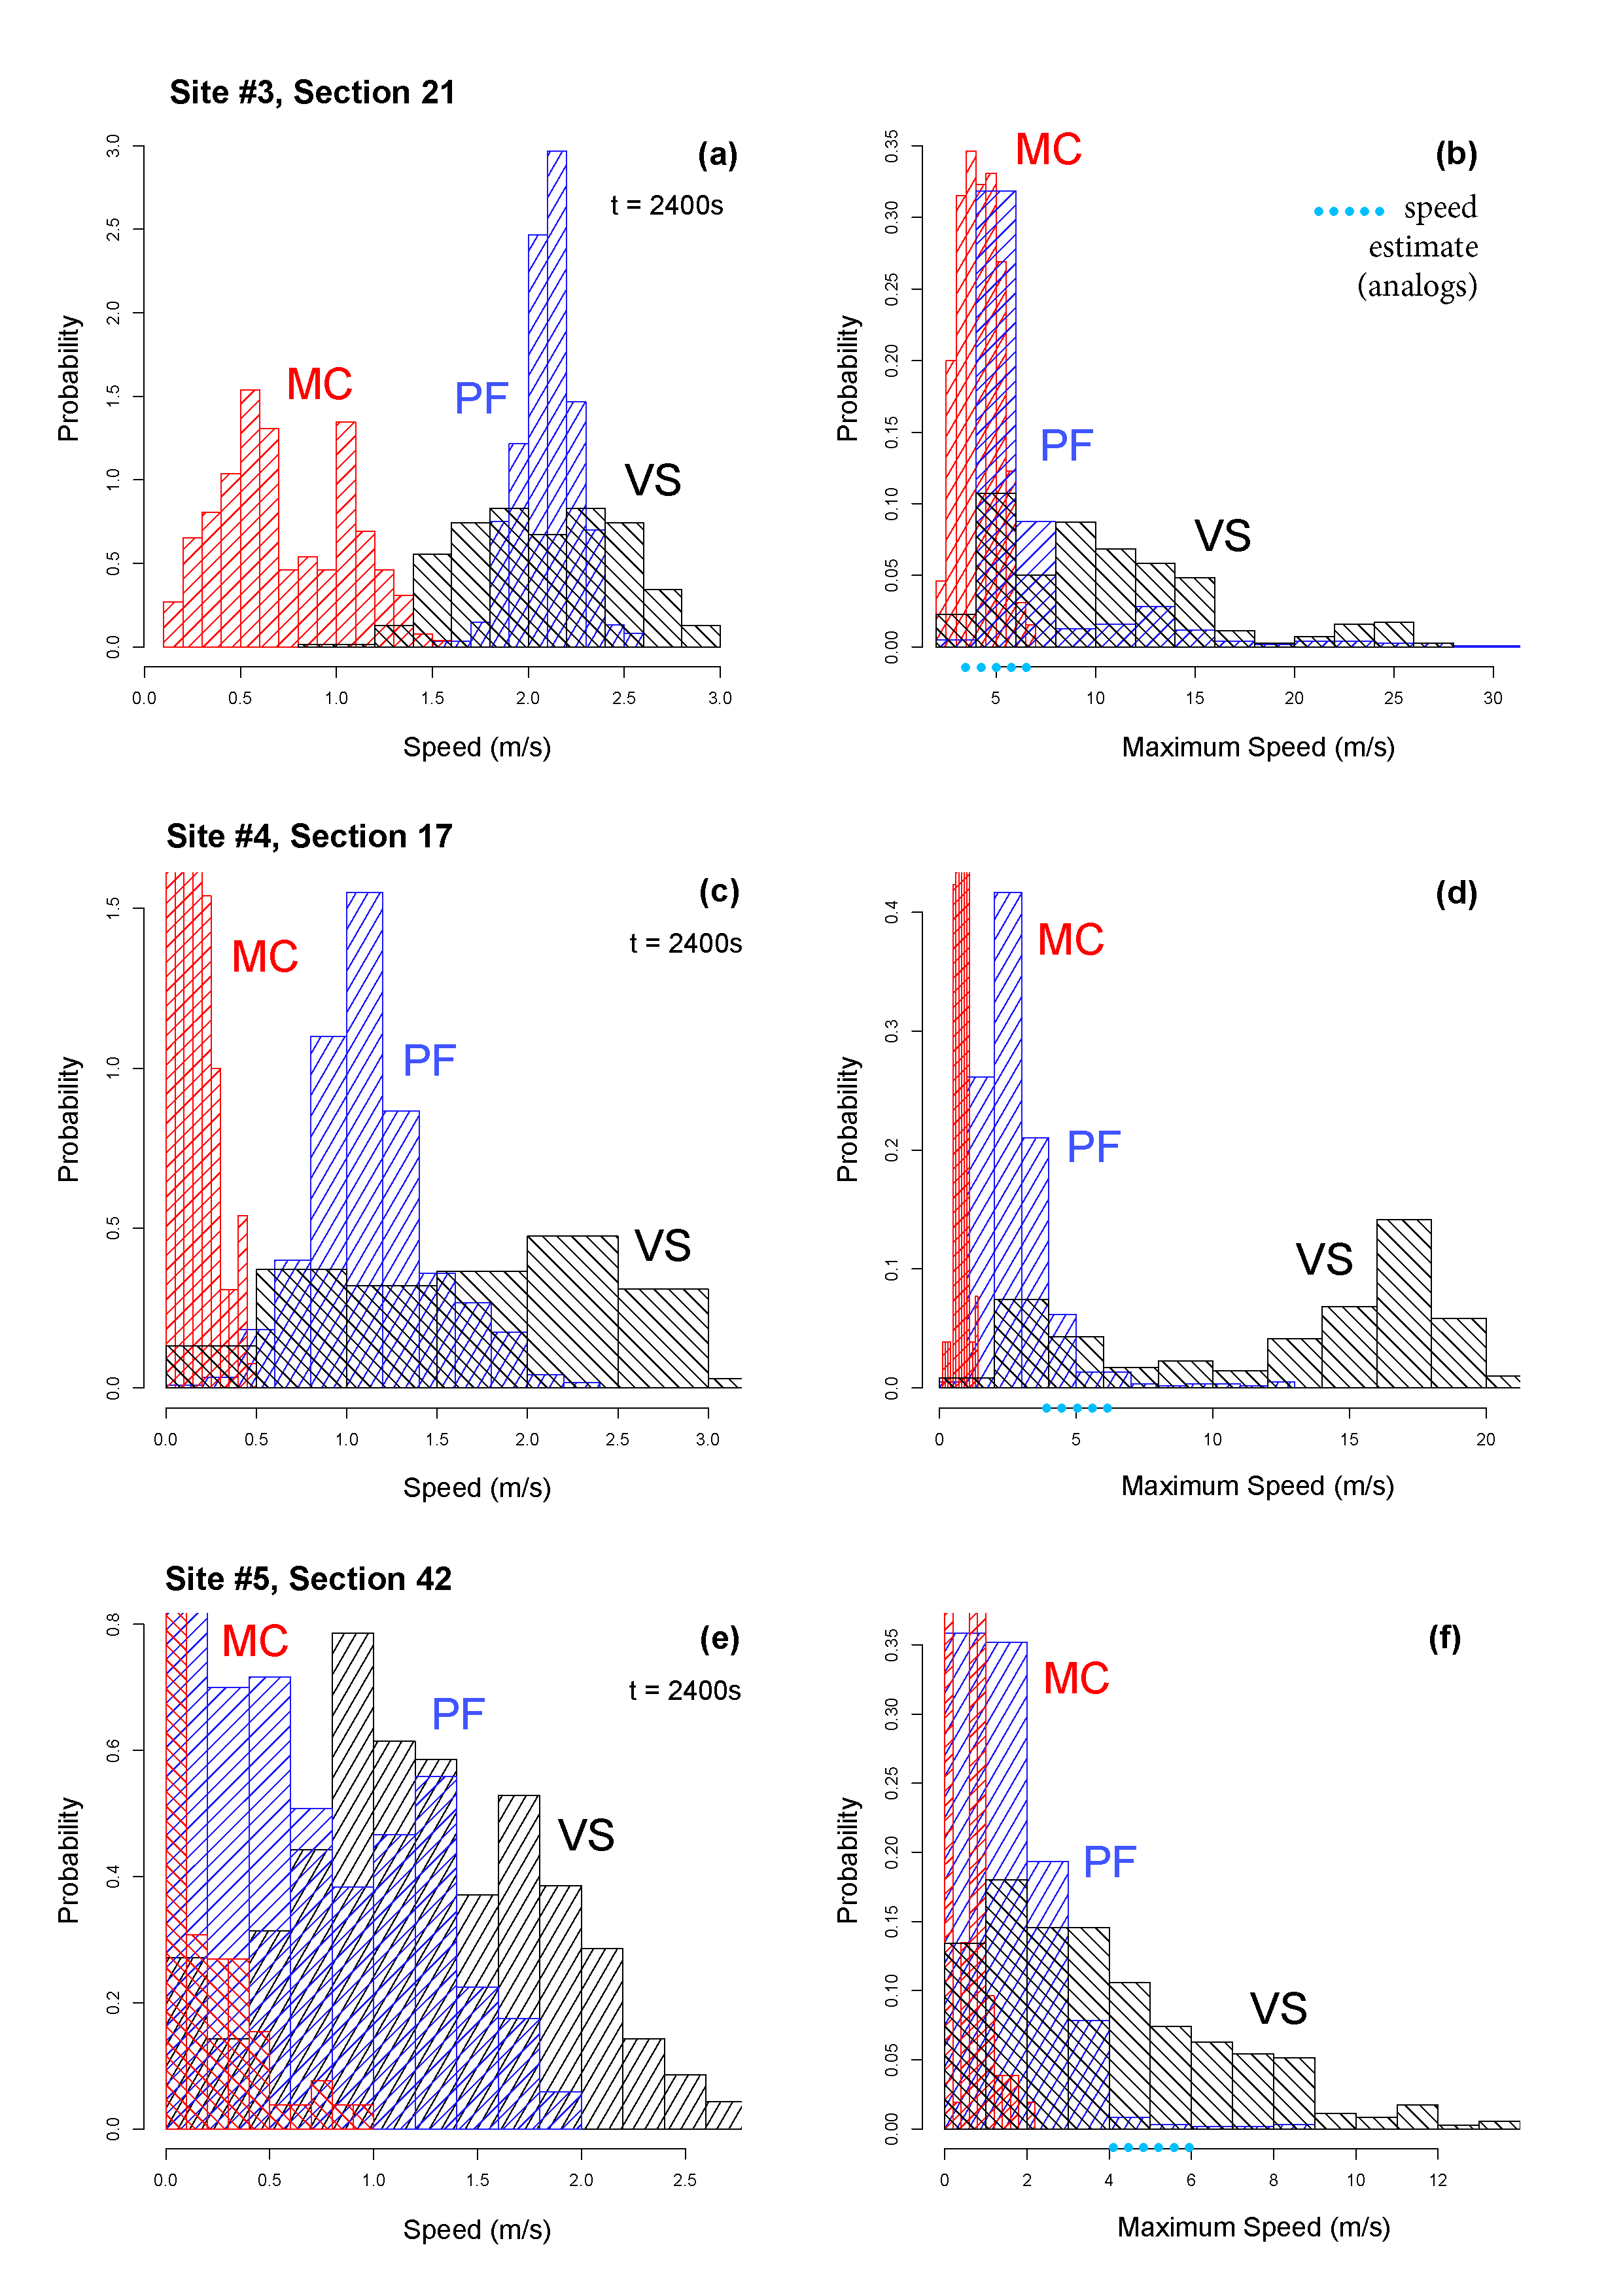
\includegraphics[width=0.8\textwidth]{Fig9.png}
\caption{...}
\label{Fig9}
\end{figure}

\subsection{Alternative performance scores of the models}

\begin{figure}[H]
\centering
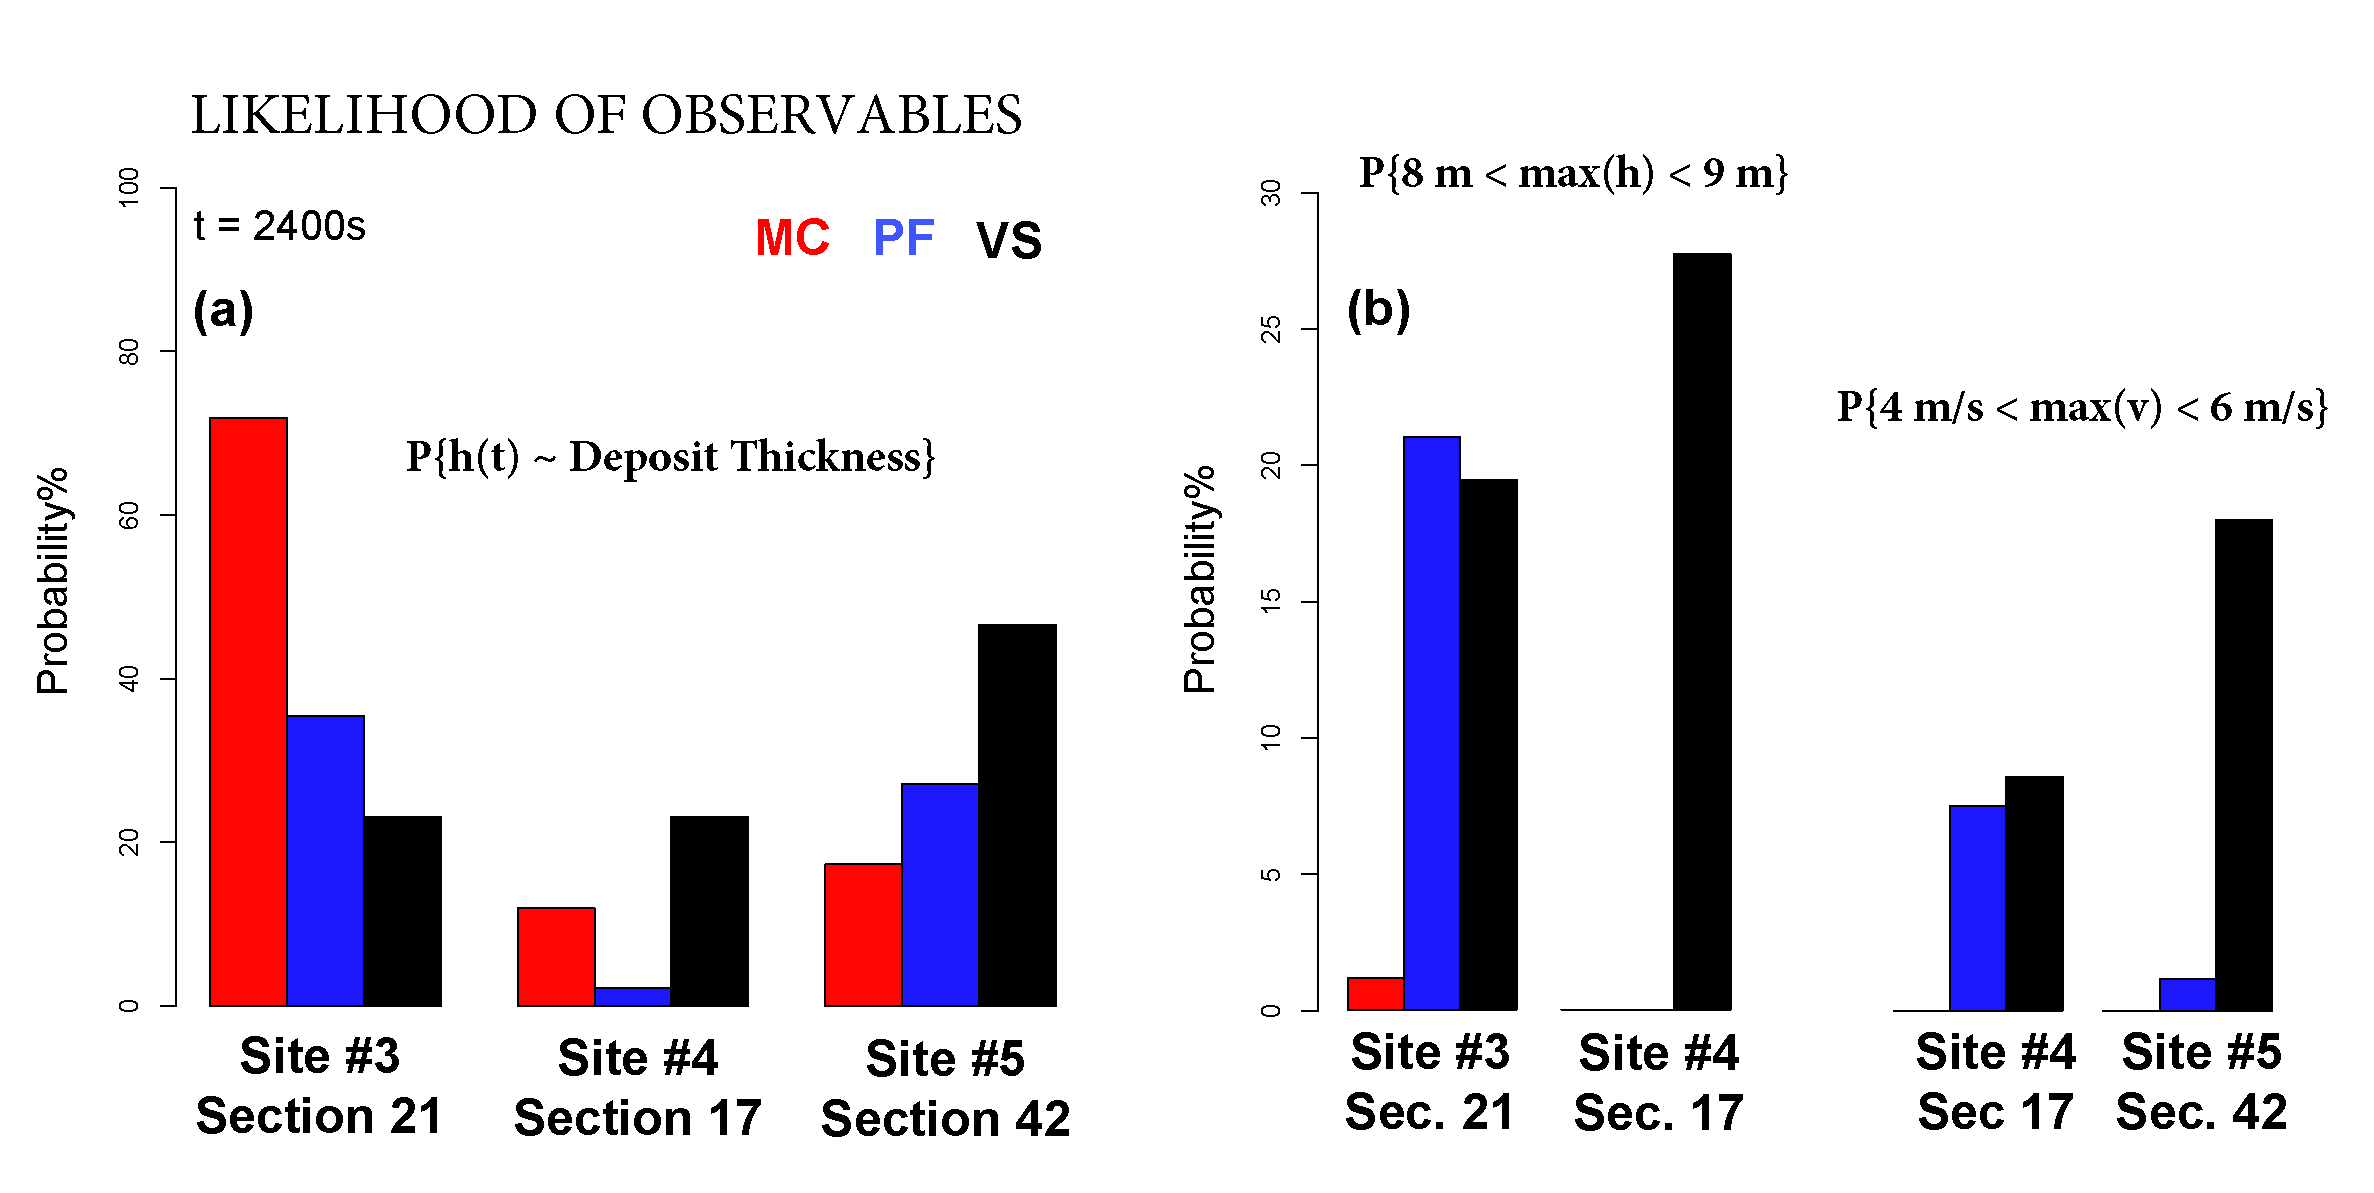
\includegraphics[width=1\textwidth]{Fig10.png}
\caption{...}
\label{Fig10}
\end{figure}

\section{Partial solutions in the specialized latin hypercube design}
\begin{figure}[H]
\centering
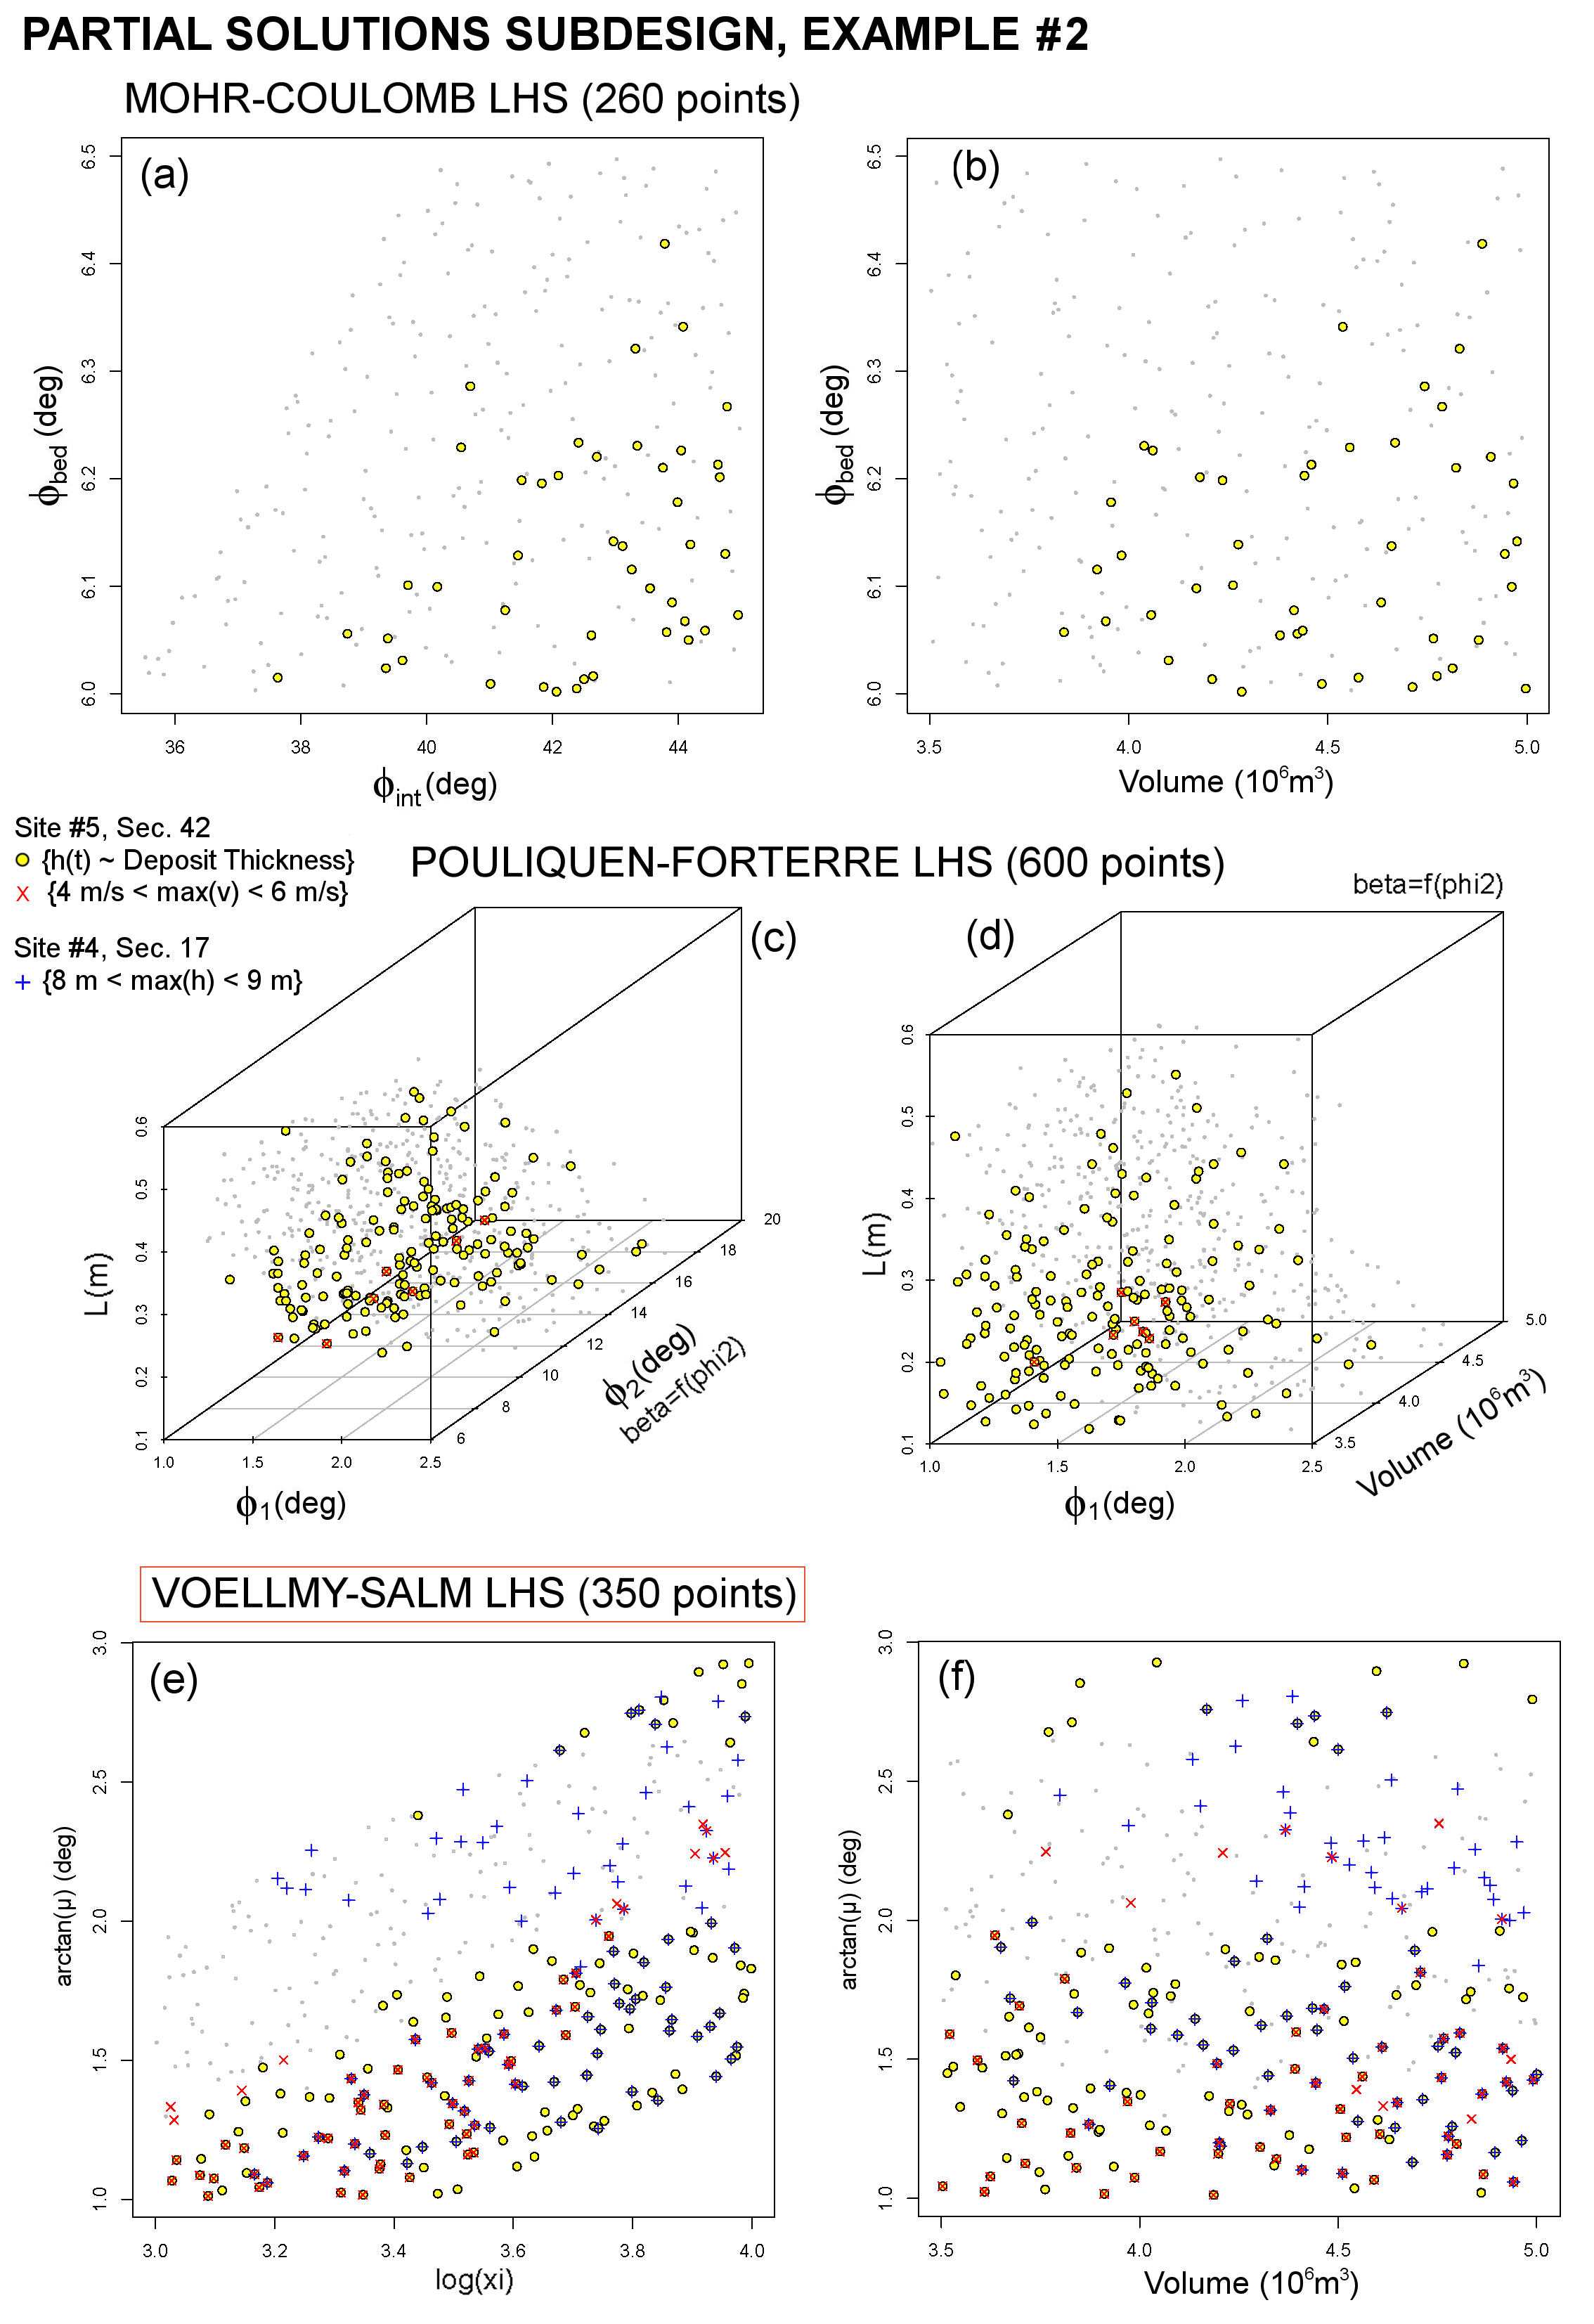
\includegraphics[width=0.8\textwidth]{Fig11.png}
\caption{...}
\label{Fig11}
\end{figure}

\begin{figure}[H]
\centering
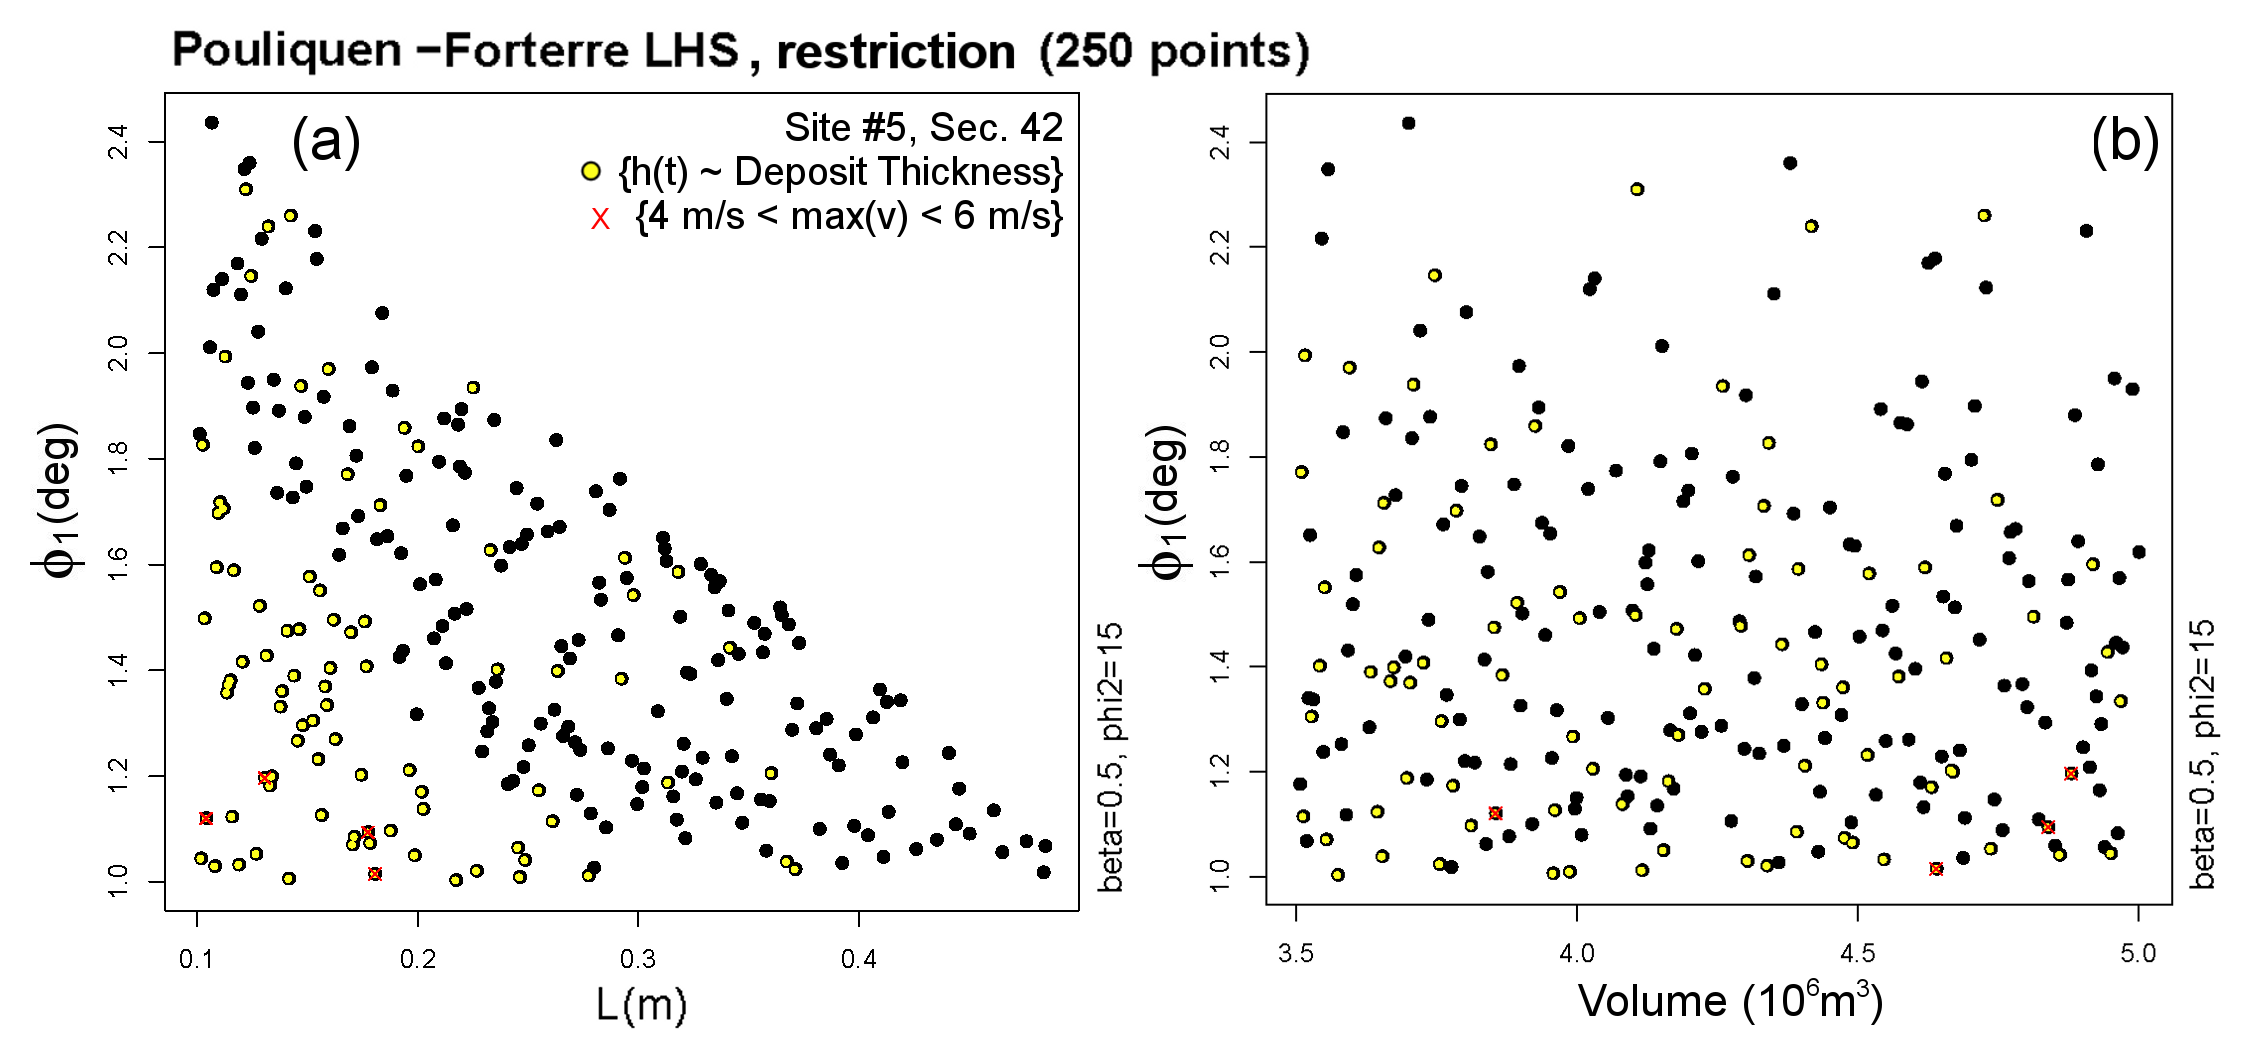
\includegraphics[width=0.8\textwidth]{FigA2.png}
\caption{...}
\label{FigA2}
\end{figure}

\subsubsection{Example of conditional results}

\begin{figure}[H]
\centering
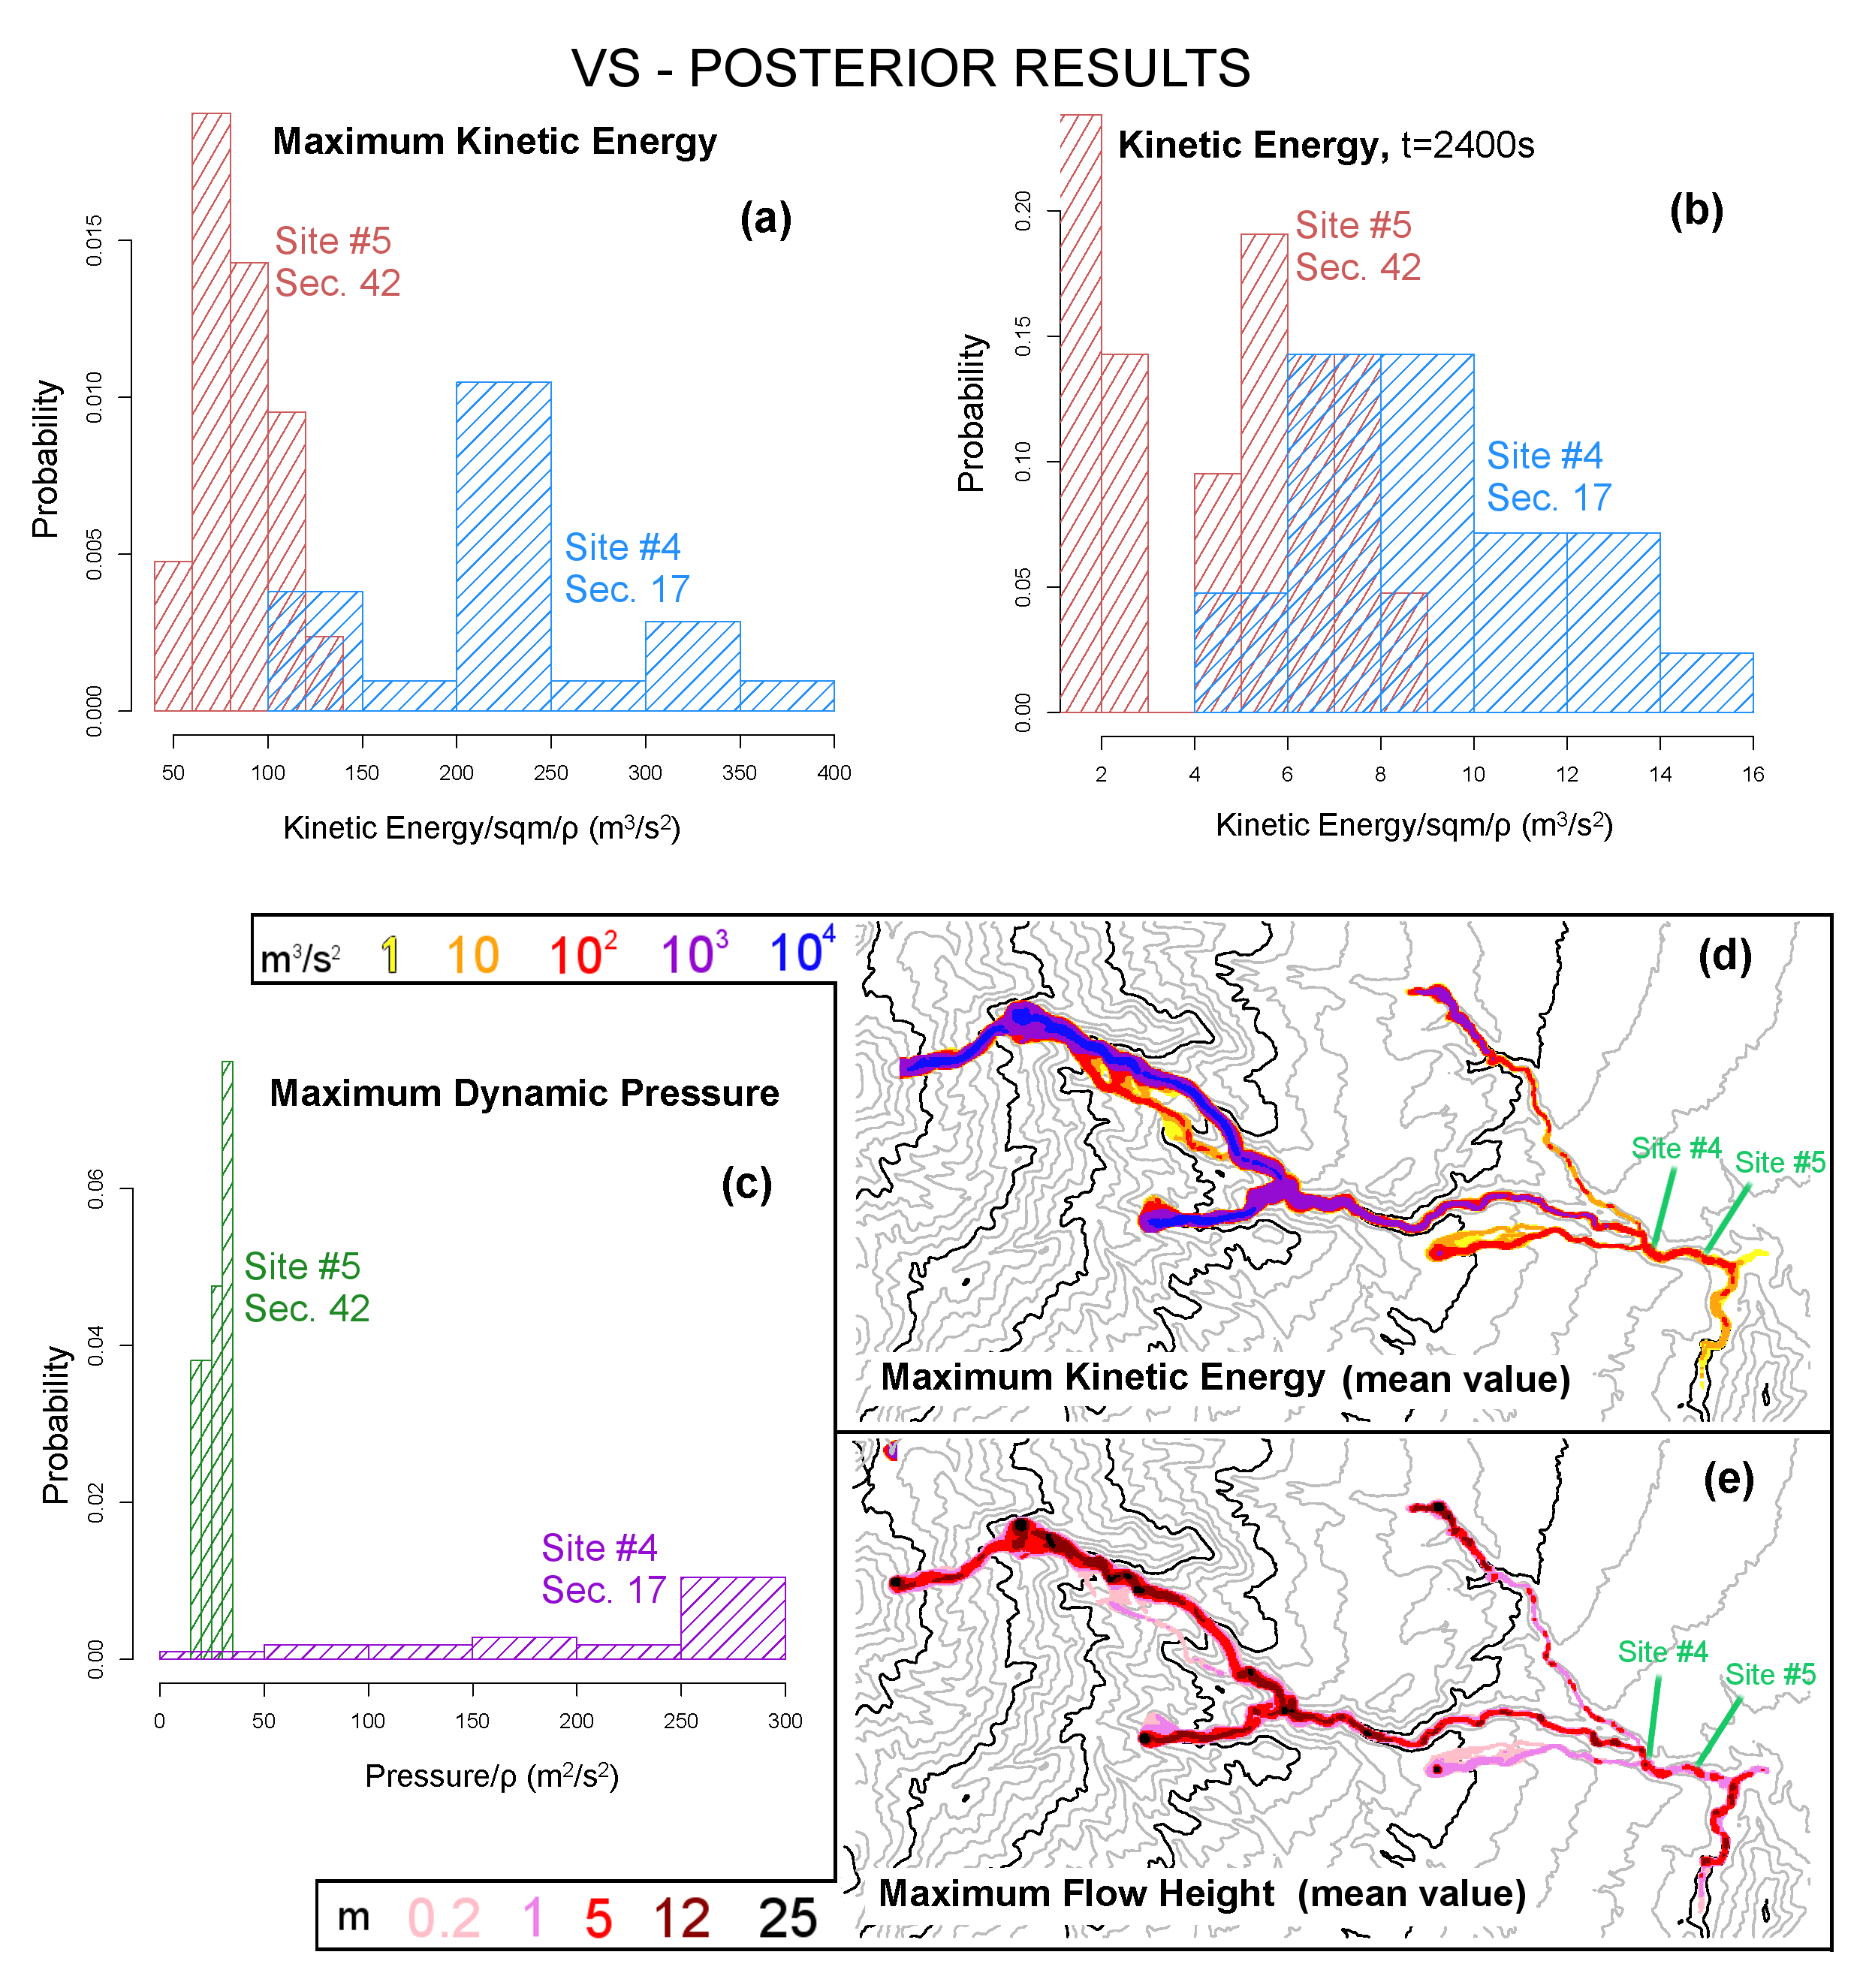
\includegraphics[width=1\textwidth]{Fig12.png}
\caption{...}
\label{Fig12}
\end{figure}

\section{Conclusions}

\section*{Acknowledgements}
We would like to acknowledge the support of NSF awards 1521855, 1621853, and 1339765.


\appendix
\section{Overview of the depth-averaged models}\label{A-1}
Models based on additional heterogeneous assumptions are possible, either more complex \citep{PitmanLe2005,Iverson2014} or more simple \citep{DadeHuppert1998}. We decided to focus on these three because of their historical relevance. We remark that the poorly constrained data available for the past flow would make the application of a more complex model very difficult.

\subsection{Mohr-Coulomb}\label{MCM}
Based on the long history of studies in soil mechanics \citep{Rankine1857,DruckerPage52}, the Mohr-Coulomb rheology (MC) was developed and used to represent the behavior of geophysical mass flows \citep{SavageHutter1989}.

Shear and normal stress are assumed to obey Coulomb friction equation, both within the flow and at its boundaries. In other words,
\begin{equation}
\tau = \sigma \tan \phi,
\end{equation}
where $\tau$ and $\sigma$ are respectively the shear and normal stresses on failure surfaces, and $\phi$ is a friction angle. This relationship does not depend on the flow speed.

We can summarize the MC rheology assumptions as:
\begin{itemize}
\item \textit{Basal Friction} based on a constant friction angle.

\item \textit{Internal Friction} based on a constant friction angle.

\item \textit{Earth pressure coefficient} formula depends on the Mohr circle (implicitly depends on the friction angles).

\item Velocity based \textit{curvature effects} are included into the equations.
\end{itemize}

Under the assumption of symmetry of the stress tensor with respect to the \textit{z} axis, the earth pressure coefficient $k=k_{ap}$ can take on only one of three values $\{ 0, \pm 1\}$. The material yield criterion is represented by the two straight lines at angles $\pm \phi$ (the internal friction angle) relative to horizontal direction. Similarly, the normal and shear stress at the bed are represented by the line $\tau=-\sigma \tan(\delta)$ where $\delta$ is the bed friction angle.

\paragraph{MC equations} As a result, we can write down the source terms of the Eqs. (\ref{eq:D_A}):
\begin{eqnarray}\label{S_terms_MC}
S_x =& g_x h  - \frac{\bar{u}}{\| \underset{^\sim}{\bar{\textbf u}} \|} \left[h\left(g_z+\frac{\bar{u}^2}{r_x}\right)\tan(\phi_{bed})\right] - h k_{ap} \ {\rm sgn}\left(\frac{\partial \bar{u}}{\partial y}\right) \frac{\partial (g_z h)}{\partial y} \sin(\phi_{int}) \nonumber \\
 S_y =& g_y h  - \frac{\bar{v}}{\| \underset{^\sim}{\bar{\textbf u}} \|} \left[h\left(g_z +\frac{\bar{v}^2}{r_y}\right)\tan(\phi_{bed})\right] - h k_{ap} \ {\rm sgn}\left({\frac{\partial \bar{v}}{\partial x}}\right) \frac{\partial (g_z h)}{\partial x} \sin(\phi_{int})
\end{eqnarray}
Where, $\underset{^\sim}{\bar{\textbf u}} = (\bar{u} , \bar{v})$, is the depth-averaged velocity vector, $r_x$ and $r_y$ denote the radii of curvature
of the local basal surface. The inverse of the radii of curvature is usually approximated with the partial derivatives of the basal slope, e.g., $1/r_x = \partial \theta_x/\partial x$, where $\theta_x$ is the local bed slope.

\subsection{Pouliquen-Forterre}\label{PFM}
The scaling properties for granular flows down rough inclined planes led to the development of the Pouliquen-Forterre rheology (PF), assuming a variable frictional behavior as a function of Froude Number and flow depth \citep{Pouliquen1999, ForterrePouliquen2002, PouliquenForterre2002, ForterrePouliquen2003}.

PF rheology assumptions can be summarized as:
\begin{itemize}
\item \textit{Basal Friction} is based on an interpolation of two different friction angles, based on the flow regime and depth.

\item \textit{Internal Friction} is neglected.

\item \textit{Earth pressure coefficient} is equal to one.

\item Normal stress is modified by a \textit{hydrostatic pressure force} related to the flow height gradient.

\item Velocity based \textit{curvature effects} are included into the equations.
\end{itemize}

Two critical slope inclination angles are defined as functions of the flow thickness, namely $\phi_{start}(h)$ and $\phi_{stop}(h)$. The function $\phi_{stop}(h)$ gives the slope angle at which a steady uniform flow leaves a deposit of thickness $h$, while $\phi_{start}(h)$ is the angle at which a layer of thickness $h$ is mobilized. They define two different basal friction coefficients.
\begin{eqnarray}
\mu_{start}(h)=\tan(\phi_{start}(h))\\
\mu_{stop}(h)=\tan(\phi_{stop}(h))
\end{eqnarray}

An empirical friction law $\mu_{b}(\|\underset{^\sim}{\bar{\textbf{u}}} \| , h)$ is then defined in the whole range of velocity and thickness. The expression changes depending on two flow regimes, according to a parameter $\beta$ and the Froude number $Fr=\| \underset{^\sim}{\bar{\textbf{u}}} \| / \ \sqrt{h g_{z}}$.

\paragraph{Dynamic friction regime - $Fr \ge \beta$}
\begin{equation}\label{mu_beta1}
\mu(h, Fr)=\mu_{stop}(h \beta / Fr)
\end{equation}

\paragraph{Intermediate friction regime - $0 \le Fr < \beta$}
\begin{equation}\label{mu_beta2}
\mu(h, Fr)=\left(\frac{Fr}{\beta}\right)^\gamma [\mu_{stop}(h)-\mu_{start}(h)] + \mu_{start}(h),
\end{equation}
where $\gamma$ is the power of extrapolation, assumed equal to $10^{-3}$ in the sequel \citep{PouliquenForterre2002}.

The functions $\mu_{stop}$ and $\mu_{start}$ are defined by:
\begin{equation}\label{mu-stop}
\mu_{stop}(h)=\tan\phi_{1} + \frac{\tan\phi_{2}-\tan\phi_{1}}{1+h/\it \mathcal{L}}
\end{equation}
and
\begin{equation}\label{mu-start}
\mu_{start}(h)=\tan\phi_{3} + \frac{\tan\phi_{2}-\tan\phi_{1}}{1+h/\it \mathcal{L}}
\end{equation}
The critical angles $\phi_{1}$, $\phi_{2}$ and $\phi_{3}$ and the parameters $\mathcal{L}, \beta$ are the parameters of the model.

In particular, $\mathcal{L}$ is the characteristic depth of the flow over which a transition between the angles $\phi_{1}$ to $\phi_{2}$ occurs, in the $\mu_{stop}$ formula. In practice, if $h\ll \mathcal L$, then $\mu_{stop}(h)\approx \tan\phi_{2}$, and if $h\gg \mathcal L$, then $\mu_{stop}(h)\approx\tan\phi_{1}$.

\paragraph{PF equations} The depth-averaged Eqs. (\ref{eq:D_A}) source terms thus take the following form:
\begin{eqnarray}\label{eq:S_terms_PF}
S_{x} &=&  g_{x} h -  \frac{\bar{u}}{\| \underset{^\sim}{\bar{\textbf{u}}} \|}\left[h \left(g_z+\frac{\bar{u}^2}{r_x}\right) \ \mu_{b}(\|\underset{^\sim}{\bar{\textbf{u}}} \| , h)\right] \ + g_{z}h\frac{\partial h}{\partial x} \nonumber \\
S_{y} &=&  g_{y} h - \frac{\bar{v}}{\| \underset{^\sim}{\bar{\textbf{u}}} \|}\left[h \left(g_z +\frac{\bar{v}^2}{r_y}\right) \ \mu_{b}(\|\underset{^\sim}{\bar{\textbf{u}}} \| , h)\right] \ + g_{z}h\frac{\partial h}{\partial y}
\end{eqnarray}

\subsection{Voellmy-Salm}\label{VSM}
The theoretical analysis of dense snow avalanches led to the VS rheology (VS) \citep{Voellmy1955, Salm1990, Salm1993, Bartelt1999}. Dense snow or debris avalanches consist of mobilized, rapidly flowing ice-snow mixed to debris-rock granules \citep{BarteltMcArdell2009}. The VS rheology assumes a velocity dependent resisting term in addition to the traditional basal friction, ideally capable of including an approximation of the turbulence-generated dissipation. Many experimental and theoretical studies were developed in this framework \citep{Gruber2007, Kern2009, Christen2010, Fischer2012}.

The following relation between shear and normal stresses holds:
\begin{equation}
\tau = \mu \sigma + \frac{\rho \| \underline{\textbf g} \|}{\xi} \| \underset{^\sim}{\bar{\textbf u}} \|^2,
\end{equation}
where, $\sigma$ denotes the normal stress at the bottom of the fluid layer and $\underline{\textbf g} = (g_{x} , g_{y} , g_{z})$ represents the gravity vector. The two parameters of the model are the bed friction coefficient $\mu$ and the velocity dependent friction coefficient $\xi$.

We can summarize VS rheology assumptions as:
\begin{itemize}
\item \textit{Basal Friction} is based on a constant coefficient, similarly to the MC rheology.

\item \textit{Internal Friction} is neglected.

\item \textit{Earth pressure coefficient} is equal to one.

\item Additional \textit{turbulent friction} is based on the local velocity by a quadratic expression.

\item Velocity based \textit{curvature effects} are included into the equations, following an alternative formulation.
\end{itemize}

The effect of the topographic local curvatures is addressed with terms containing the local radii of curvature $r_x$ and $r_y$. In this case the expression is based on the speed instead of the scalar components of velocity \citep{PudasainiHutter2003,Fischer2012}.

\paragraph{VS equations} Therefore, the final source terms take the following form:
\begin{eqnarray}
\label{eq:S_terms_VS}
S_{x} &=&  g_{x} h - \frac{\bar{u}}{\| \underset{^\sim}{\bar{\textbf u}}\|} \ \left[ h \left(g_{z} + \frac{\| \underset{^\sim}{\bar{\textbf u}} \|^2}{r_{x}} \right)\mu+ \frac{\| \underset{^\sim}{\textbf g} \|}{\xi}\| \underset{^\sim}{\bar{\textbf u}} \|^2\right], \nonumber \\
S_{y} &=& g_{y} h - \frac{\bar{v}}{\| \underset{^\sim}{\bar{\textbf u}}\|} \ \left[ h \left(g_{z} + \frac{\| \underset{^\sim}{\bar{\textbf u}} \|^2}{r_{y}} \right)\mu+ \frac{\| \underset{^\sim}{\textbf g} \|}{\xi}\| \underset{^\sim}{\bar{\textbf u}} \|^2\right].
\end{eqnarray}

\section{Contribution variables}\label{A-2}
Let $(F_i(\underline{\textbf x},t))_{i=1,\dots, 4}$ be an array of force terms, where $\underline{\textbf x}\in \mathbf R^d$ is a spatial location, and $t\in T$ is a time instant. The degree of contribution of those force terms to the flow dynamics can be significantly variable in space and time, and we define the \emph{dominance factors} $[p_j(\underline{\textbf x},t)]_{j=1,\dots, k}$, i.e., the probability of each $F_j(\underline{\textbf x},t)$ to be the dominant force. Those probabilities provide insight into the dominance of a particular source or dissipation term on the model dynamics. We remark that we focus on the modulus of the forces and hence we cope with scalar terms. It is also important to remark that all the forces depend on the input variables, and they can be thus considered as random variables. Furthermore, these definitions are general and could be applied to any set of contributing variables, and not only to the force terms. More details about this can be found in \cite{Patra2018}.

\begin{definition}[Dominance factors]
Let $(F_i)_{i\in I}$ be random variables on $(\Omega, \mathcal F, P_M)$. Then, $\forall i$, the dominant variable is defined as:
$$\Phi:=\left\{
    \begin{array}{ll}
      \max_i |F_i|, & \hbox{if not null;} \\
      1, & \hbox{otherwise.}
    \end{array}
  \right.$$
In particular, for each $j \in I$, the dominance factors are defined as:
$$p_j:=P_M\left\{\Phi=|F_j|\right\}.$$
\end{definition}

Moreover, we define the \emph{random contributions}, an additional tool that we use to compare the different force terms, following a less restrictive approach than the dominance factors. They are obtained dividing the force terms by the dominant force $\Phi$, and hence belong to $[0,1]$.

\begin{definition}[Expected contributions]
Let $(F_i)_{i\in I}$ be random variables on $(\Omega, \mathcal F, P_M)$. Then, $\forall i$, the random contribution is defined as:
$$C_i:=\frac{F_i}{\Phi},$$
where $\Phi$ is the dominant variable. Thus, $\forall i$, the expected contributions are defined by $E\left[C_i\right]$.
\end{definition}

In particular, for a particular location $x$, time $t$, and parameter sample $\omega$, we have $C_i(\underline{\textbf x},t,\omega)=0$ if there is no flow or all the forces are null. The expectation of $C_i$ is reduced by the chance of $F_i$ being small compared to the other terms, or by the chance of having no flow in $(\underline{\textbf x},t)$.

\bibliographystyle{apalike}
\bibliography{mybibfileMX}
\end{document}

